\documentclass[a4paper, 12pt]{article}
\usepackage[T1]{fontenc}
\usepackage[utf8]{inputenc}

\usepackage[a4paper]{geometry}
\usepackage{titlesec}
\usepackage{amsmath}
\usepackage{amsfonts}
\usepackage{amsthm}
\usepackage{xcolor}
\usepackage[bottom]{footmisc}
\usepackage[colorlinks=true, linkcolor=blue, citecolor=red, urlcolor=violet]{hyperref}
\usepackage{graphicx}
\usepackage{subcaption}
\usepackage{caption}


% FIGURES can be defined here and then used or directly defined within the text
\def\FigureOne{\centering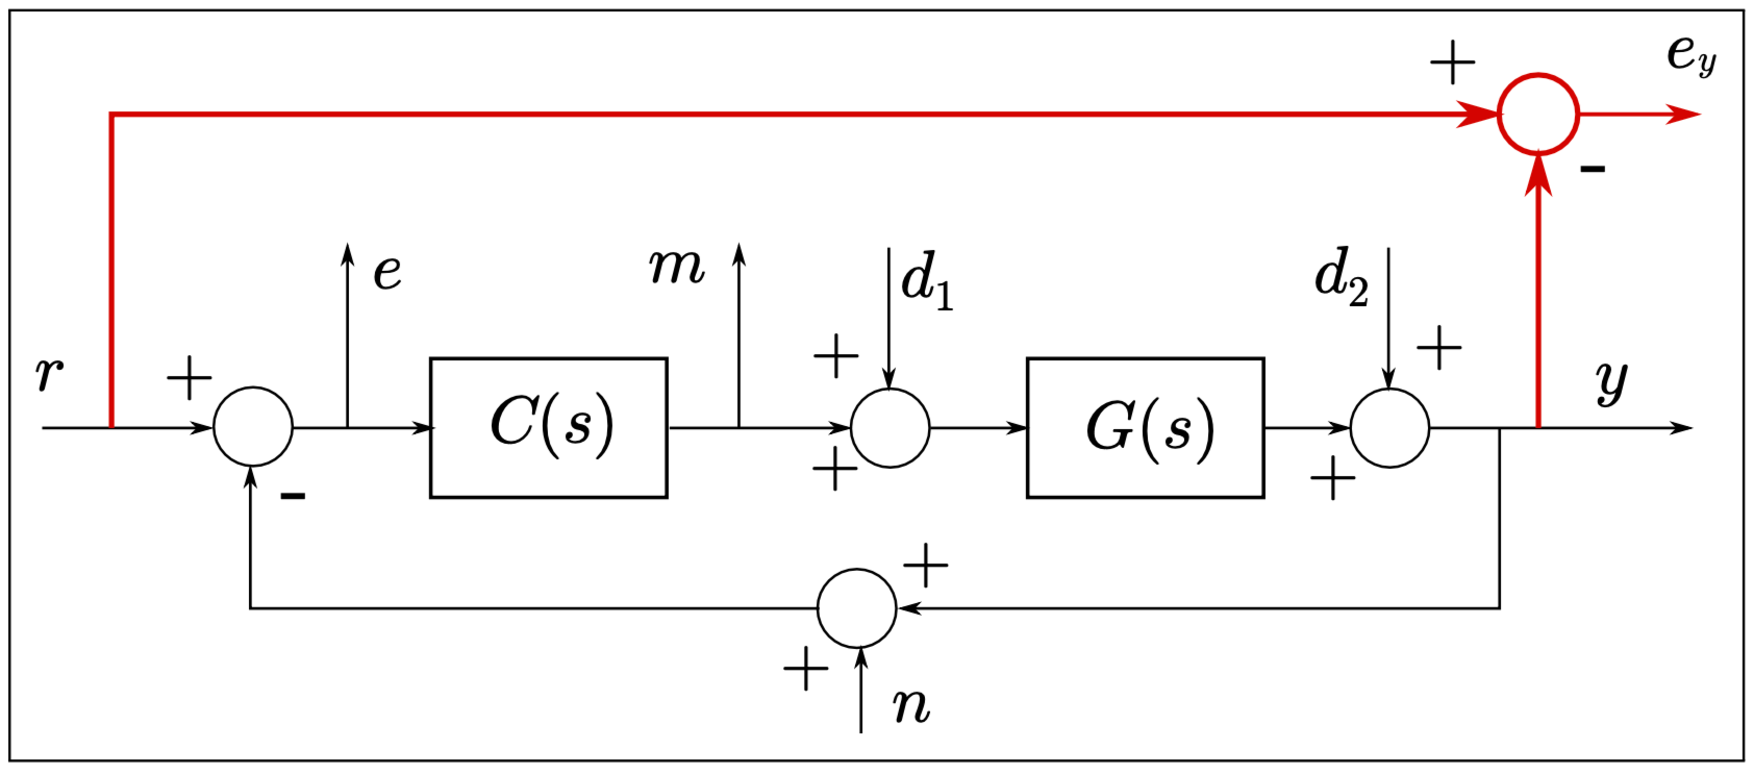
\includegraphics[width=0.5\textwidth]{Figures/fig01.pdf}}

\def\FigureTwo{\centering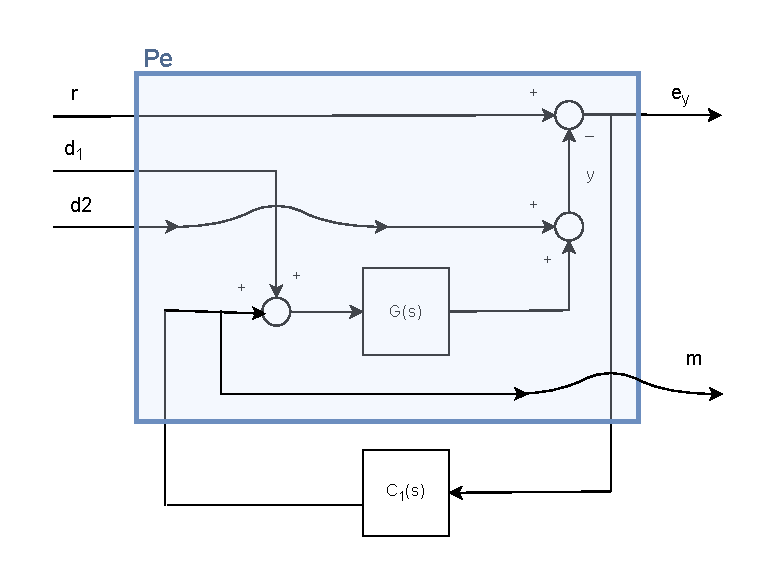
\includegraphics[width=0.5\textwidth]{Figures/fig02.pdf}}

\def\FigureThreeA{\centering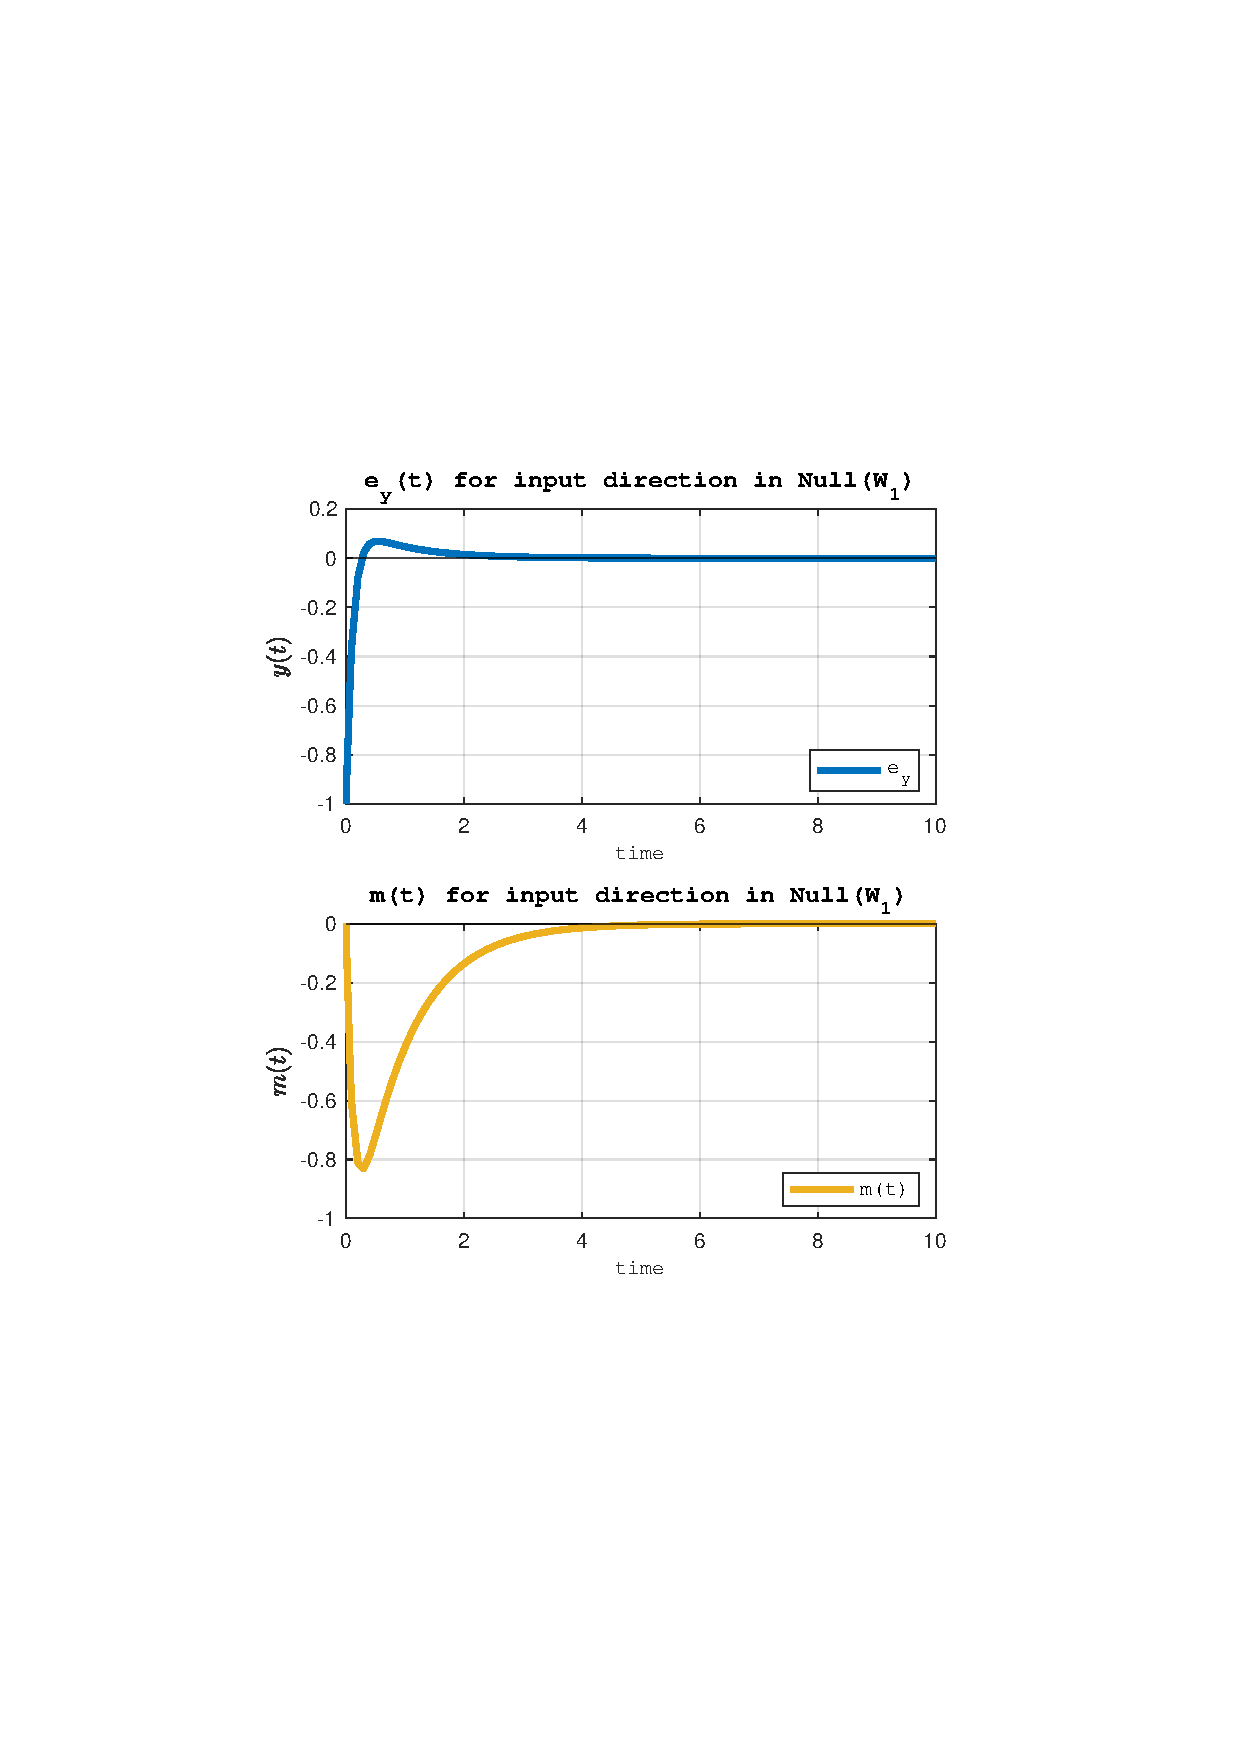
\includegraphics[width=0.3\textwidth]{Figures/fig03a.pdf}}

\def\FigureThreeB{\centering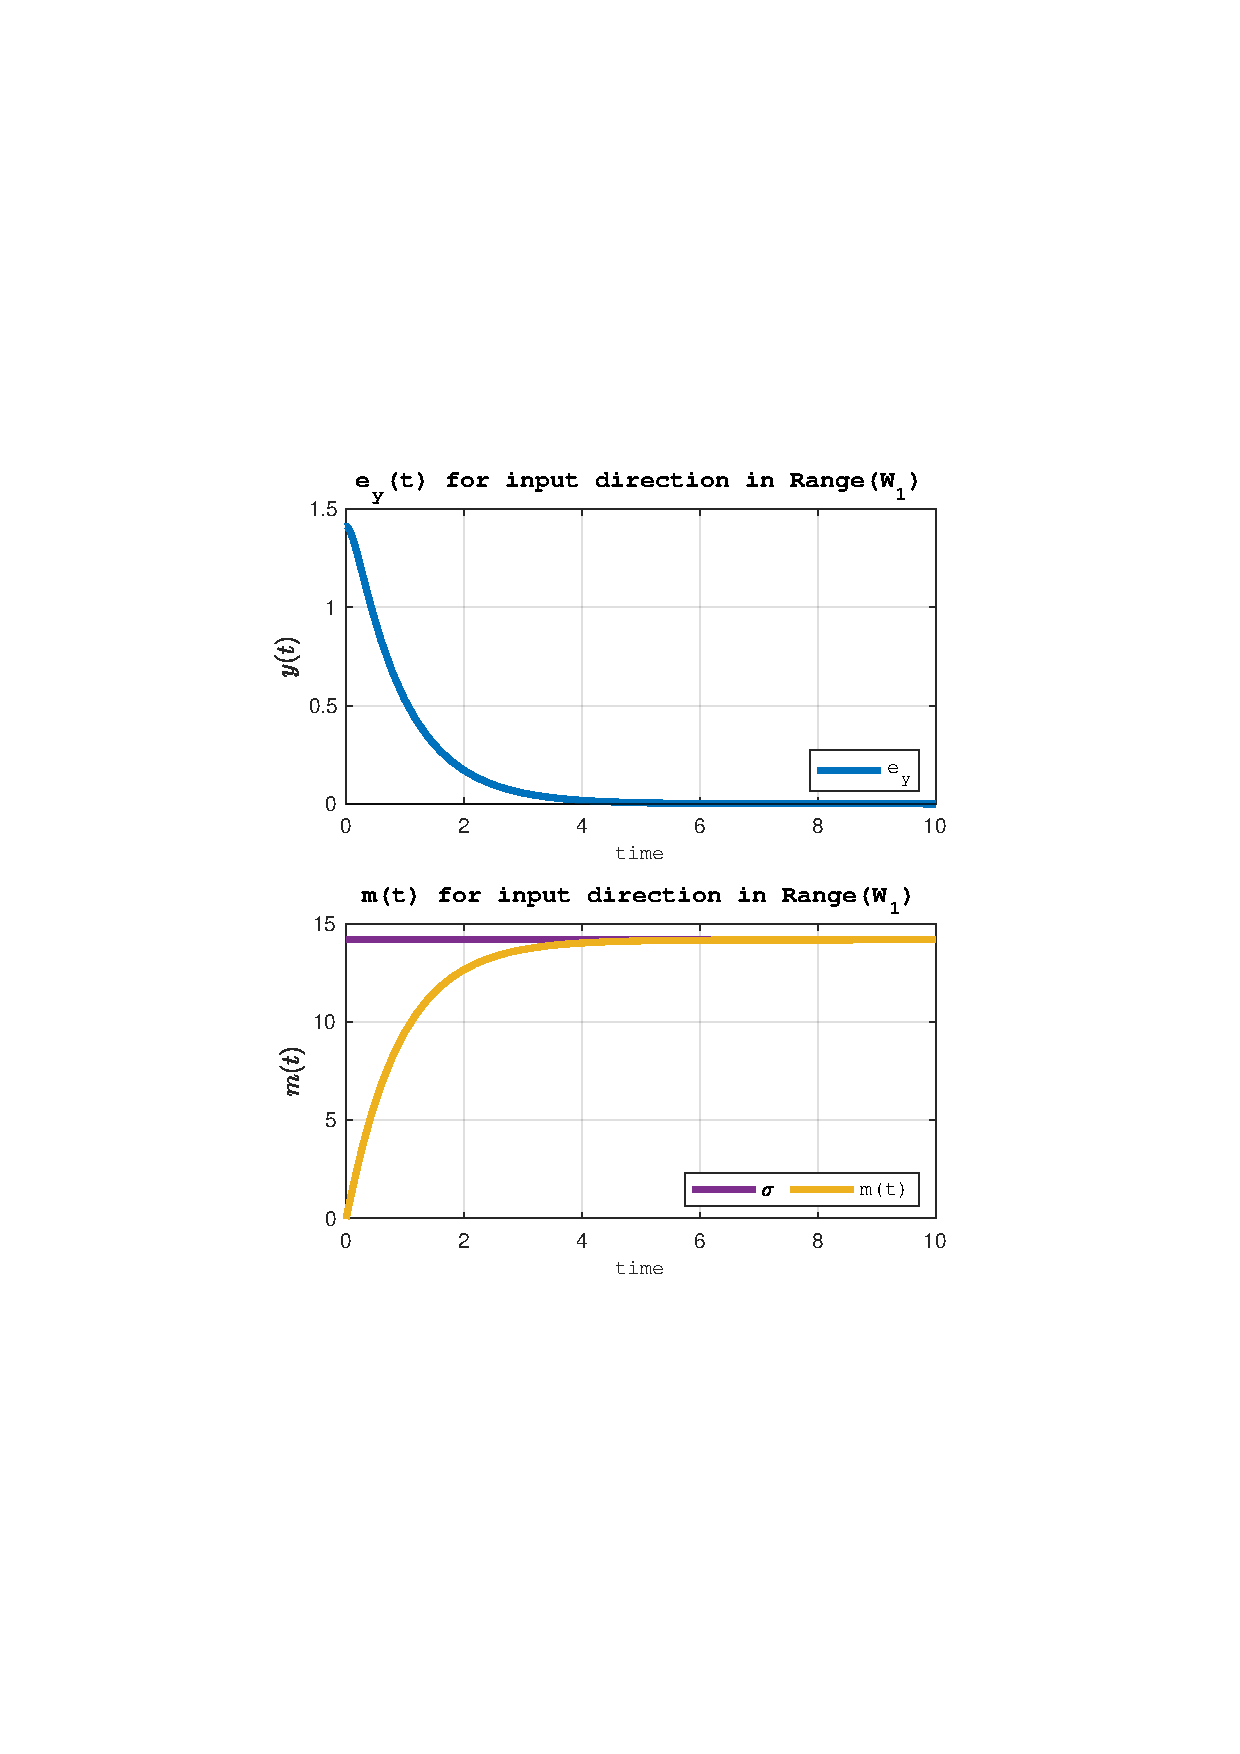
\includegraphics[width=0.3\textwidth]{Figures/fig03b.pdf}}

\def\FigureThreeC{\centering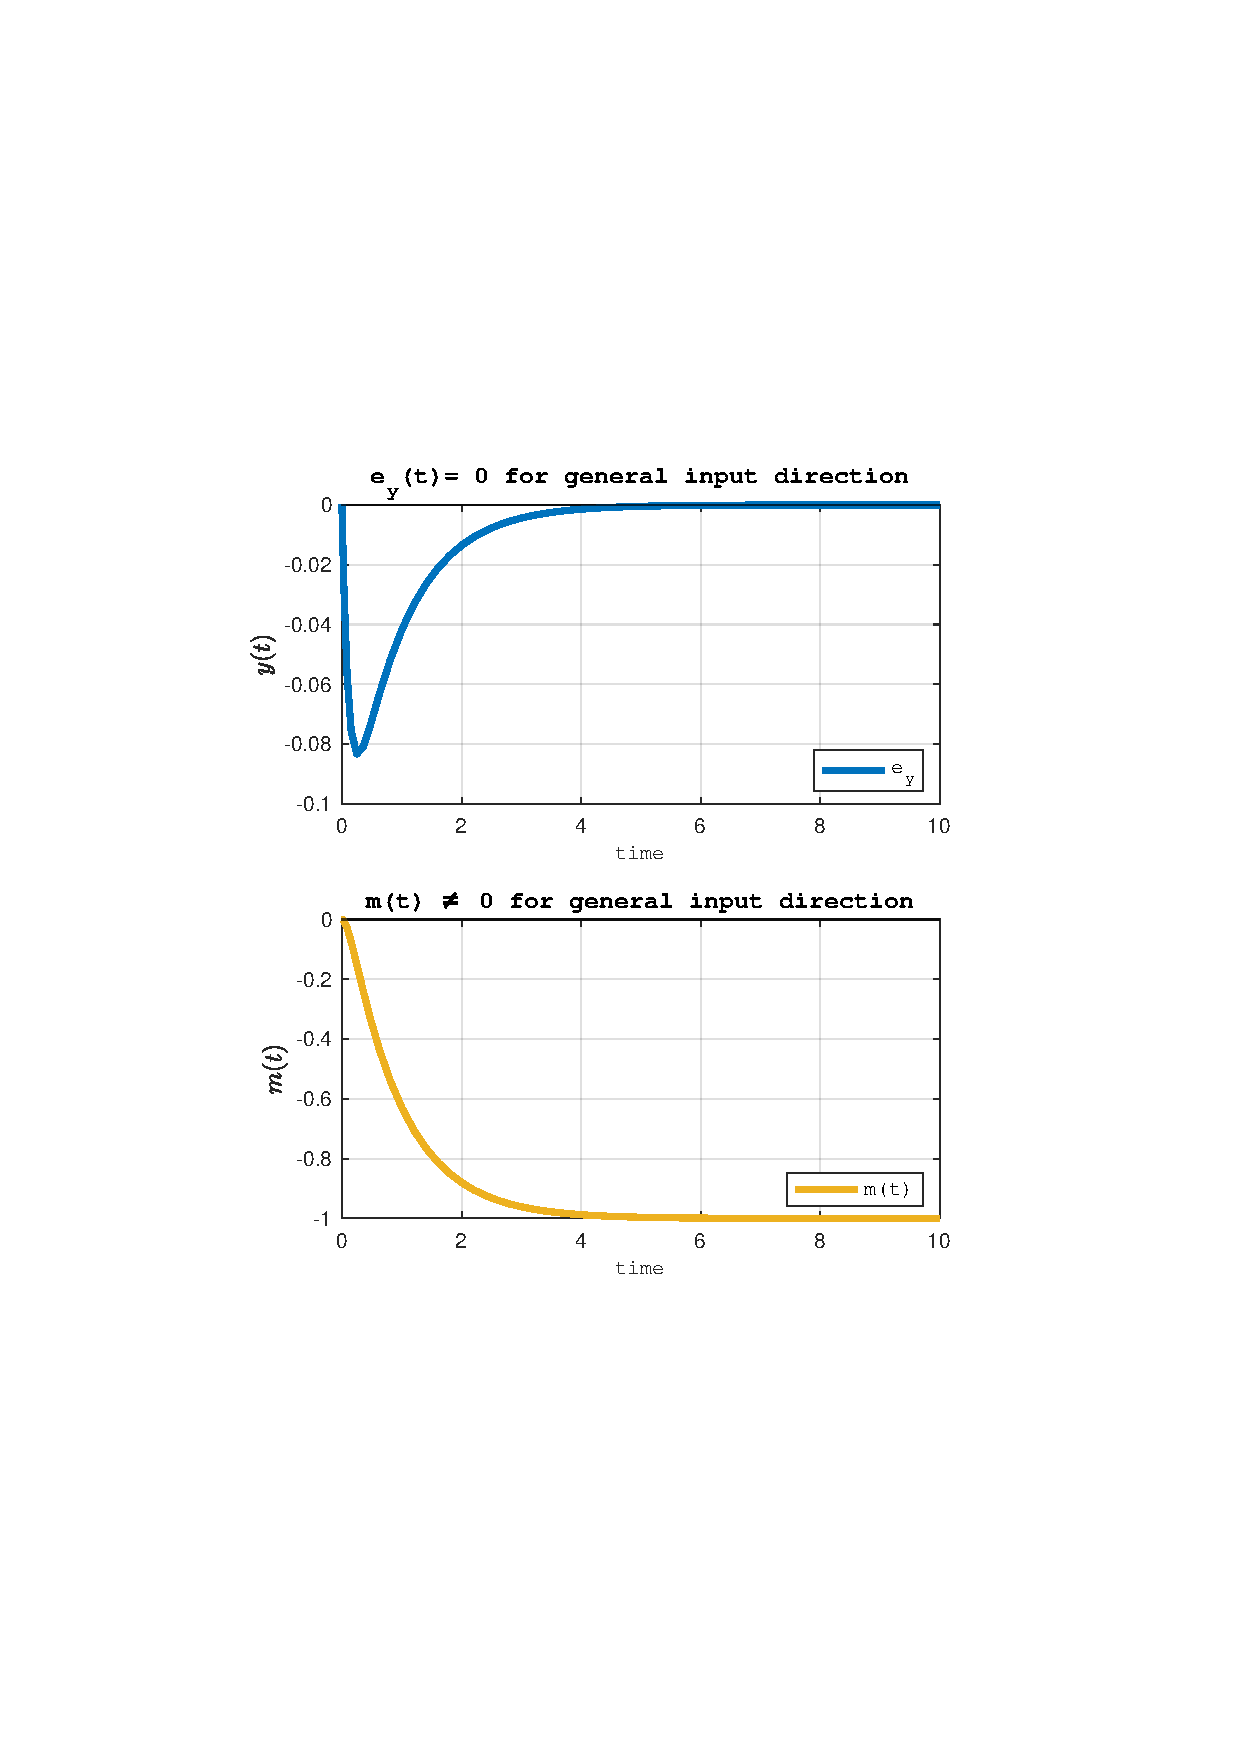
\includegraphics[width=0.3\textwidth]{Figures/fig03c.pdf}}

\def\FigureFour{\centering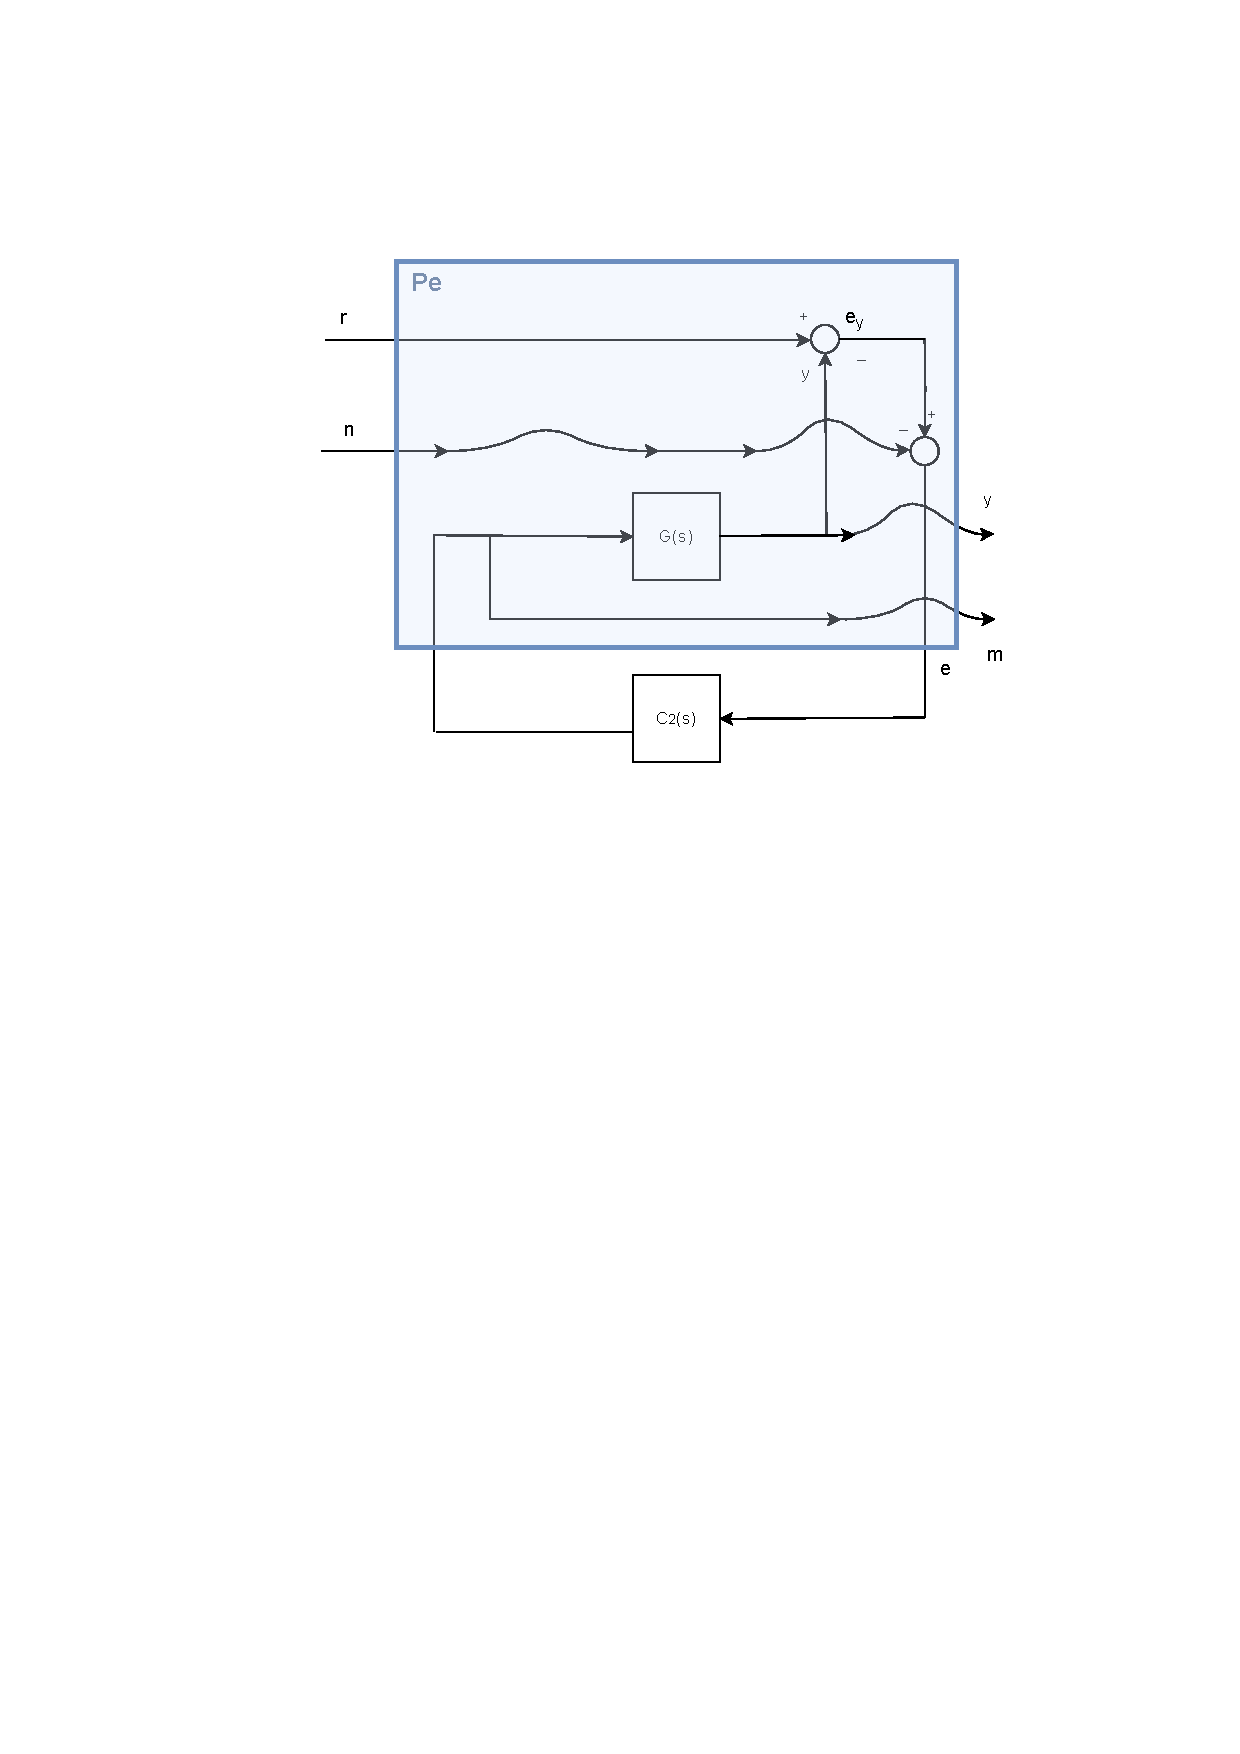
\includegraphics[width=0.6\textwidth]{Figures/fig04.pdf}}

\def\FigureFive{\centering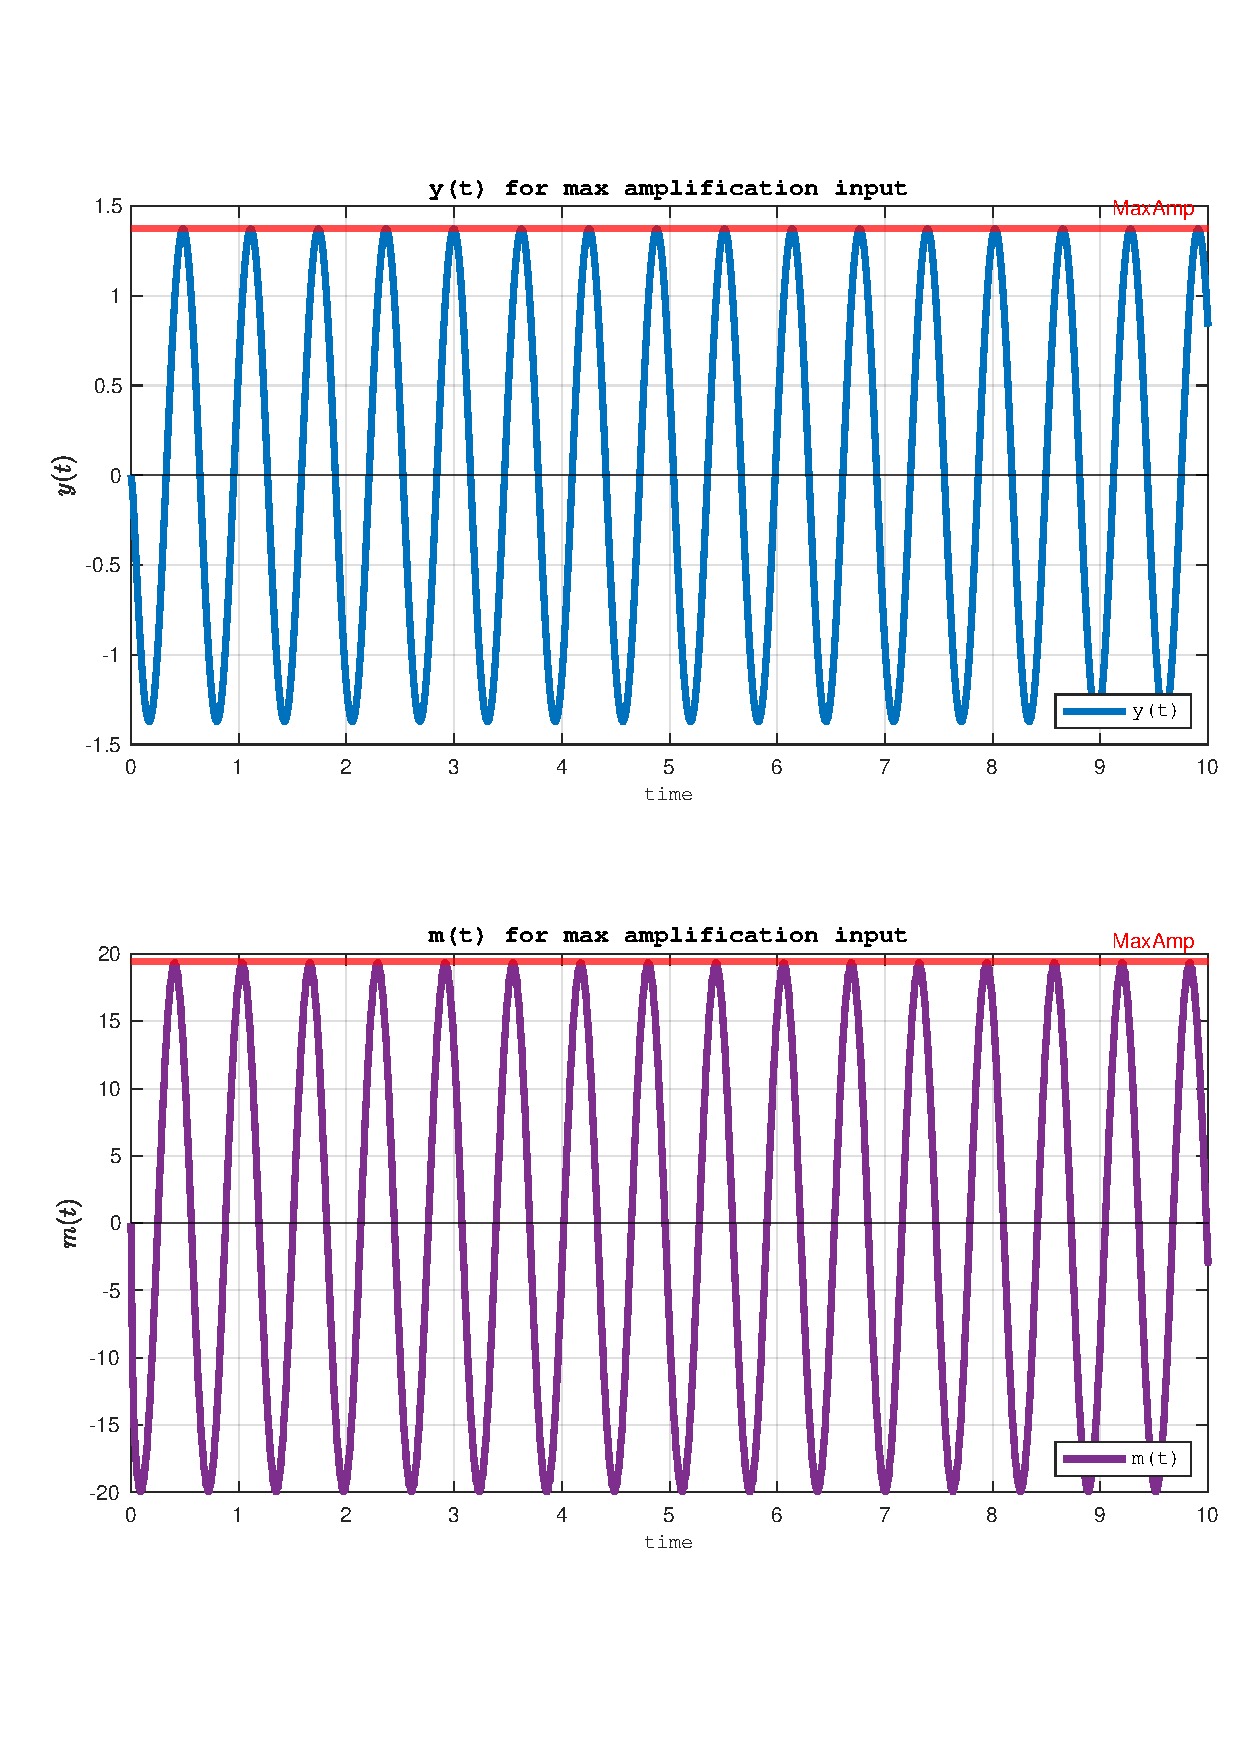
\includegraphics[width=0.8\textwidth]{Figures/fig05.pdf}}

\def\FigureSix{\centering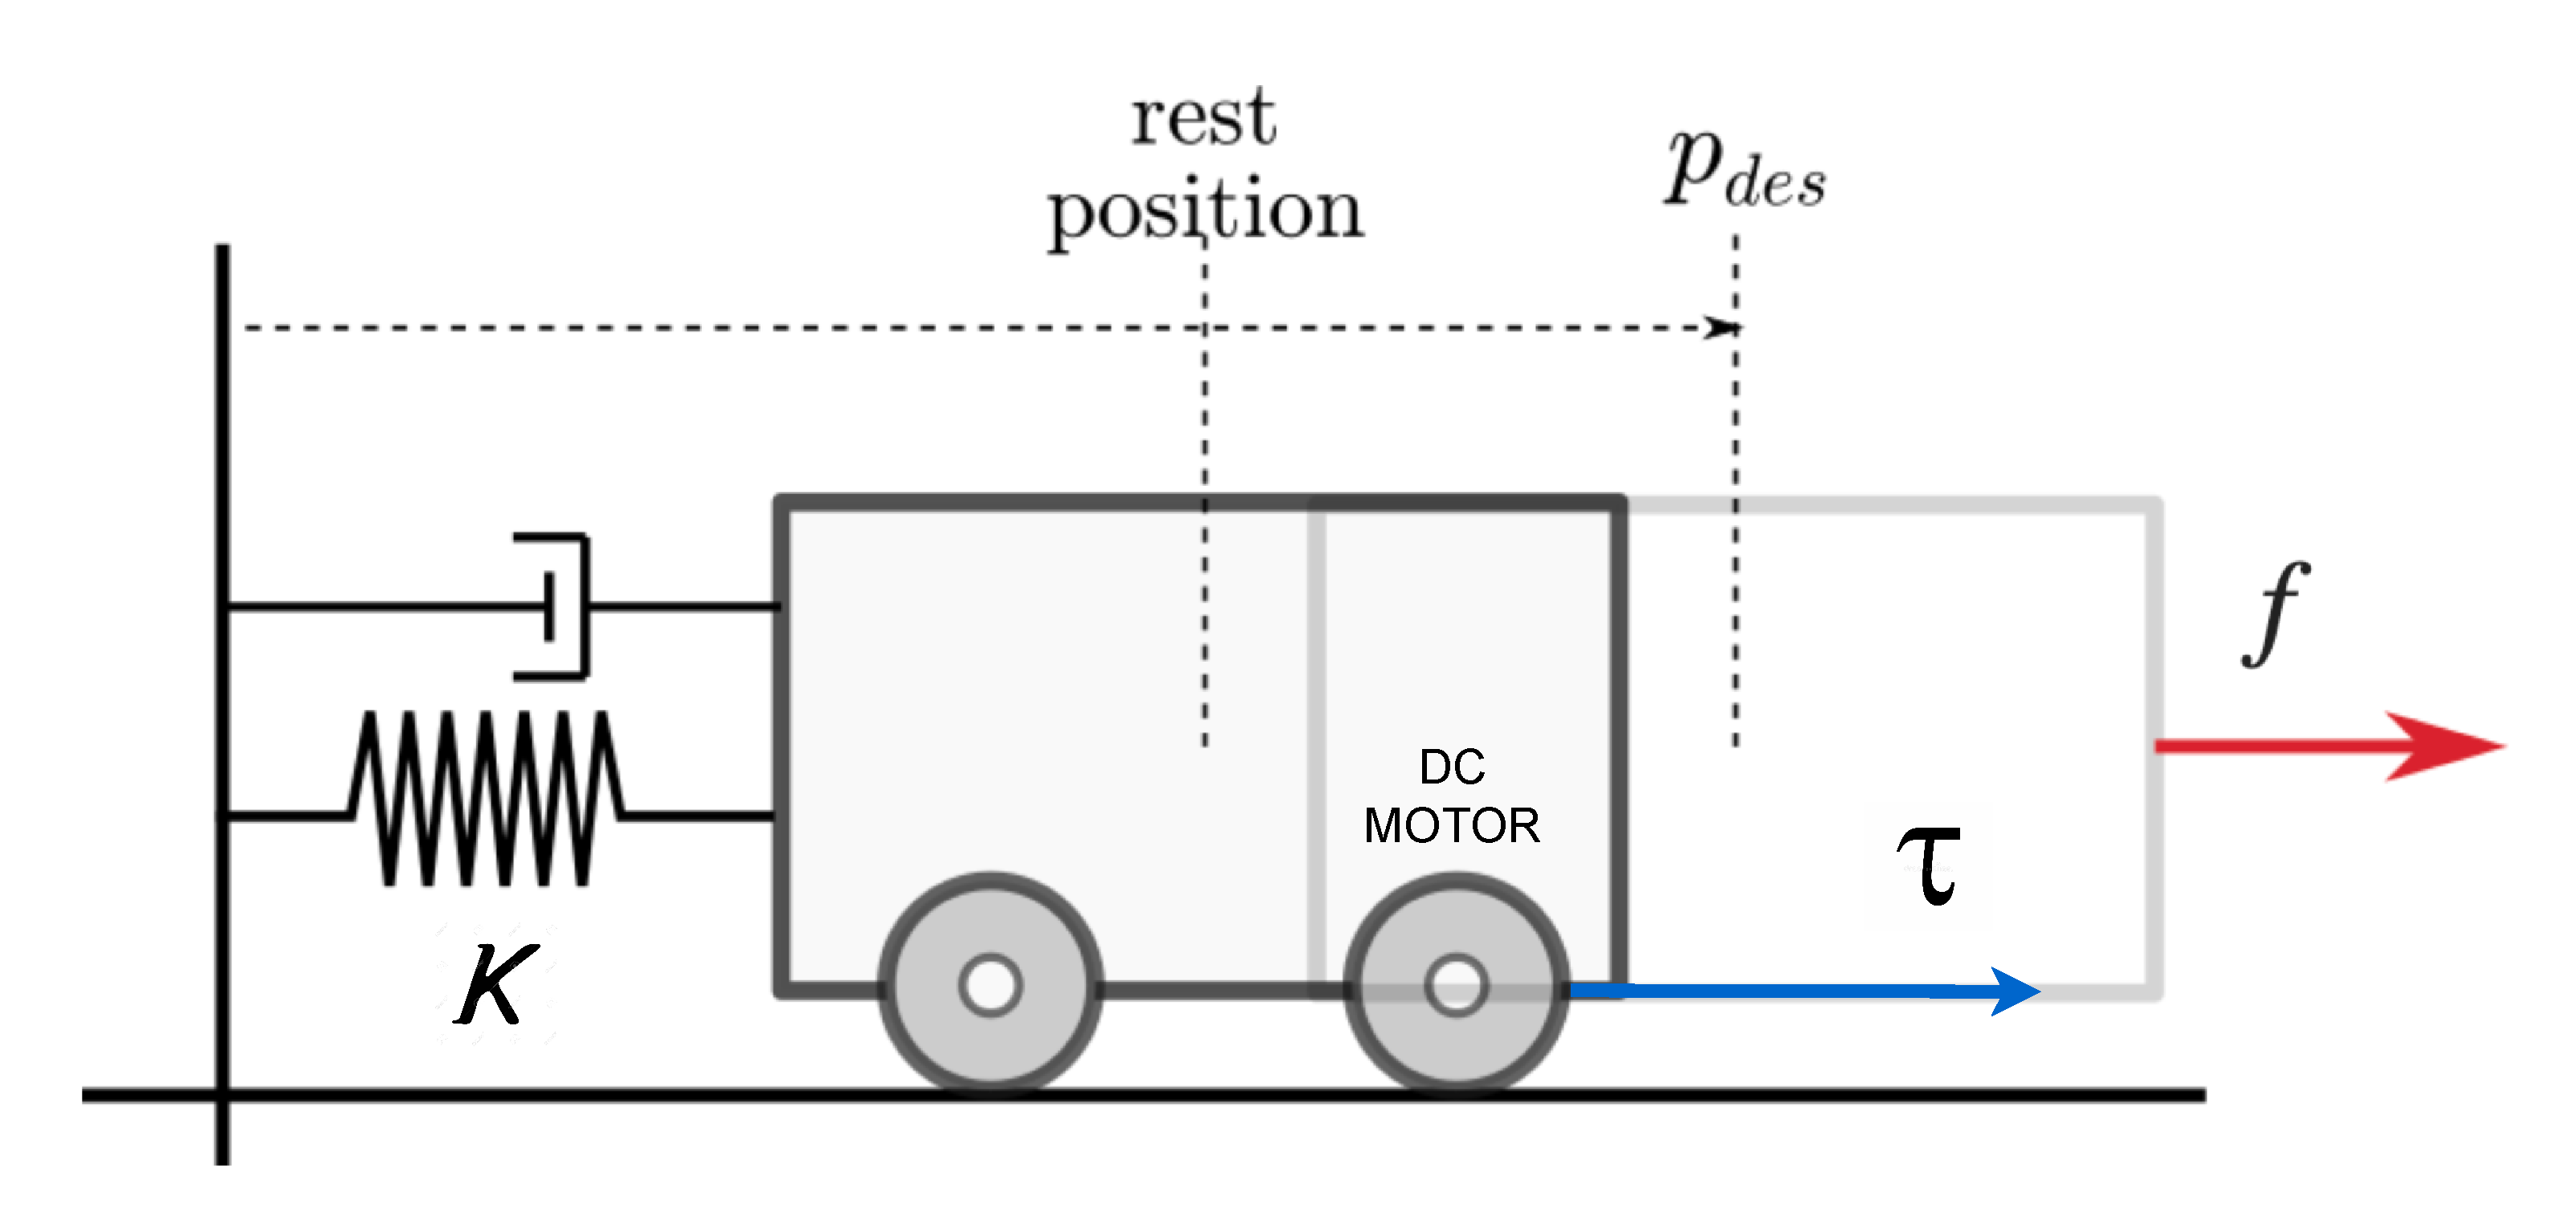
\includegraphics[width=0.8\textwidth]{Figures/fig06.pdf}}

\def\FigureSeven{\centering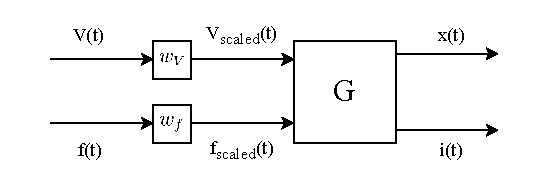
\includegraphics[width=0.8\textwidth]{Figures/fig07.pdf}}

\def\FigureAugmented{\centering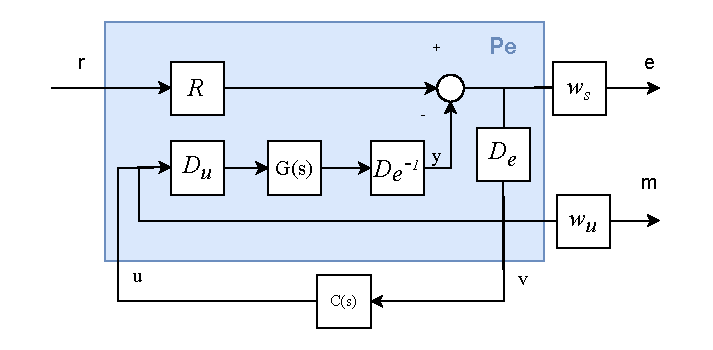
\includegraphics[width=0.8\textwidth]{Figures/2I2Oc.pdf}}

\def\FigureEight{\centering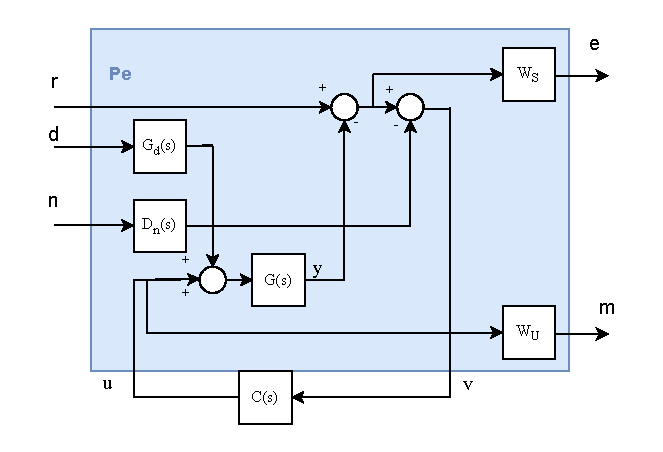
\includegraphics[width=0.7\textwidth]{Figures/fig08.pdf}}

\def\FigureEleven{\centering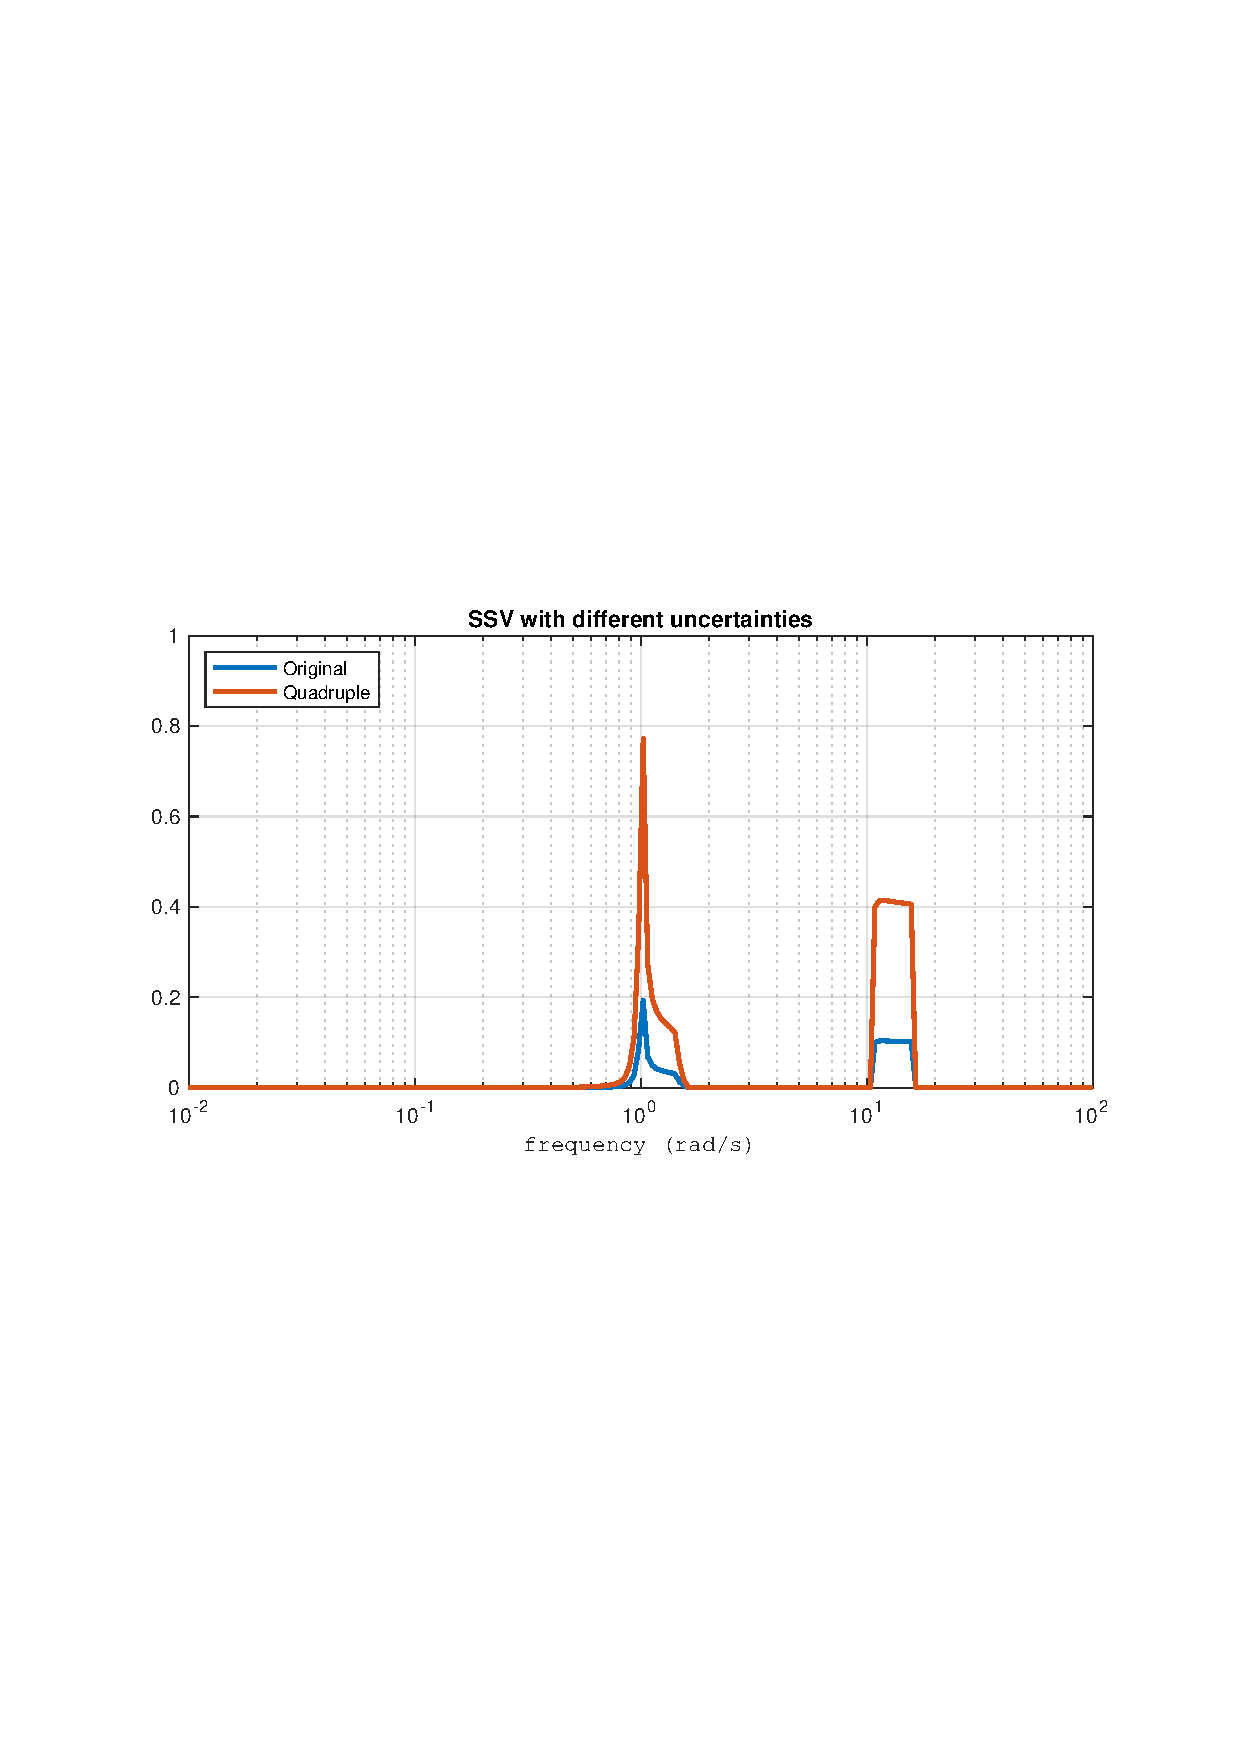
\includegraphics[width=0.7\textwidth]{Figures/fig11.pdf}}

\def\FigureTwelveA{\centering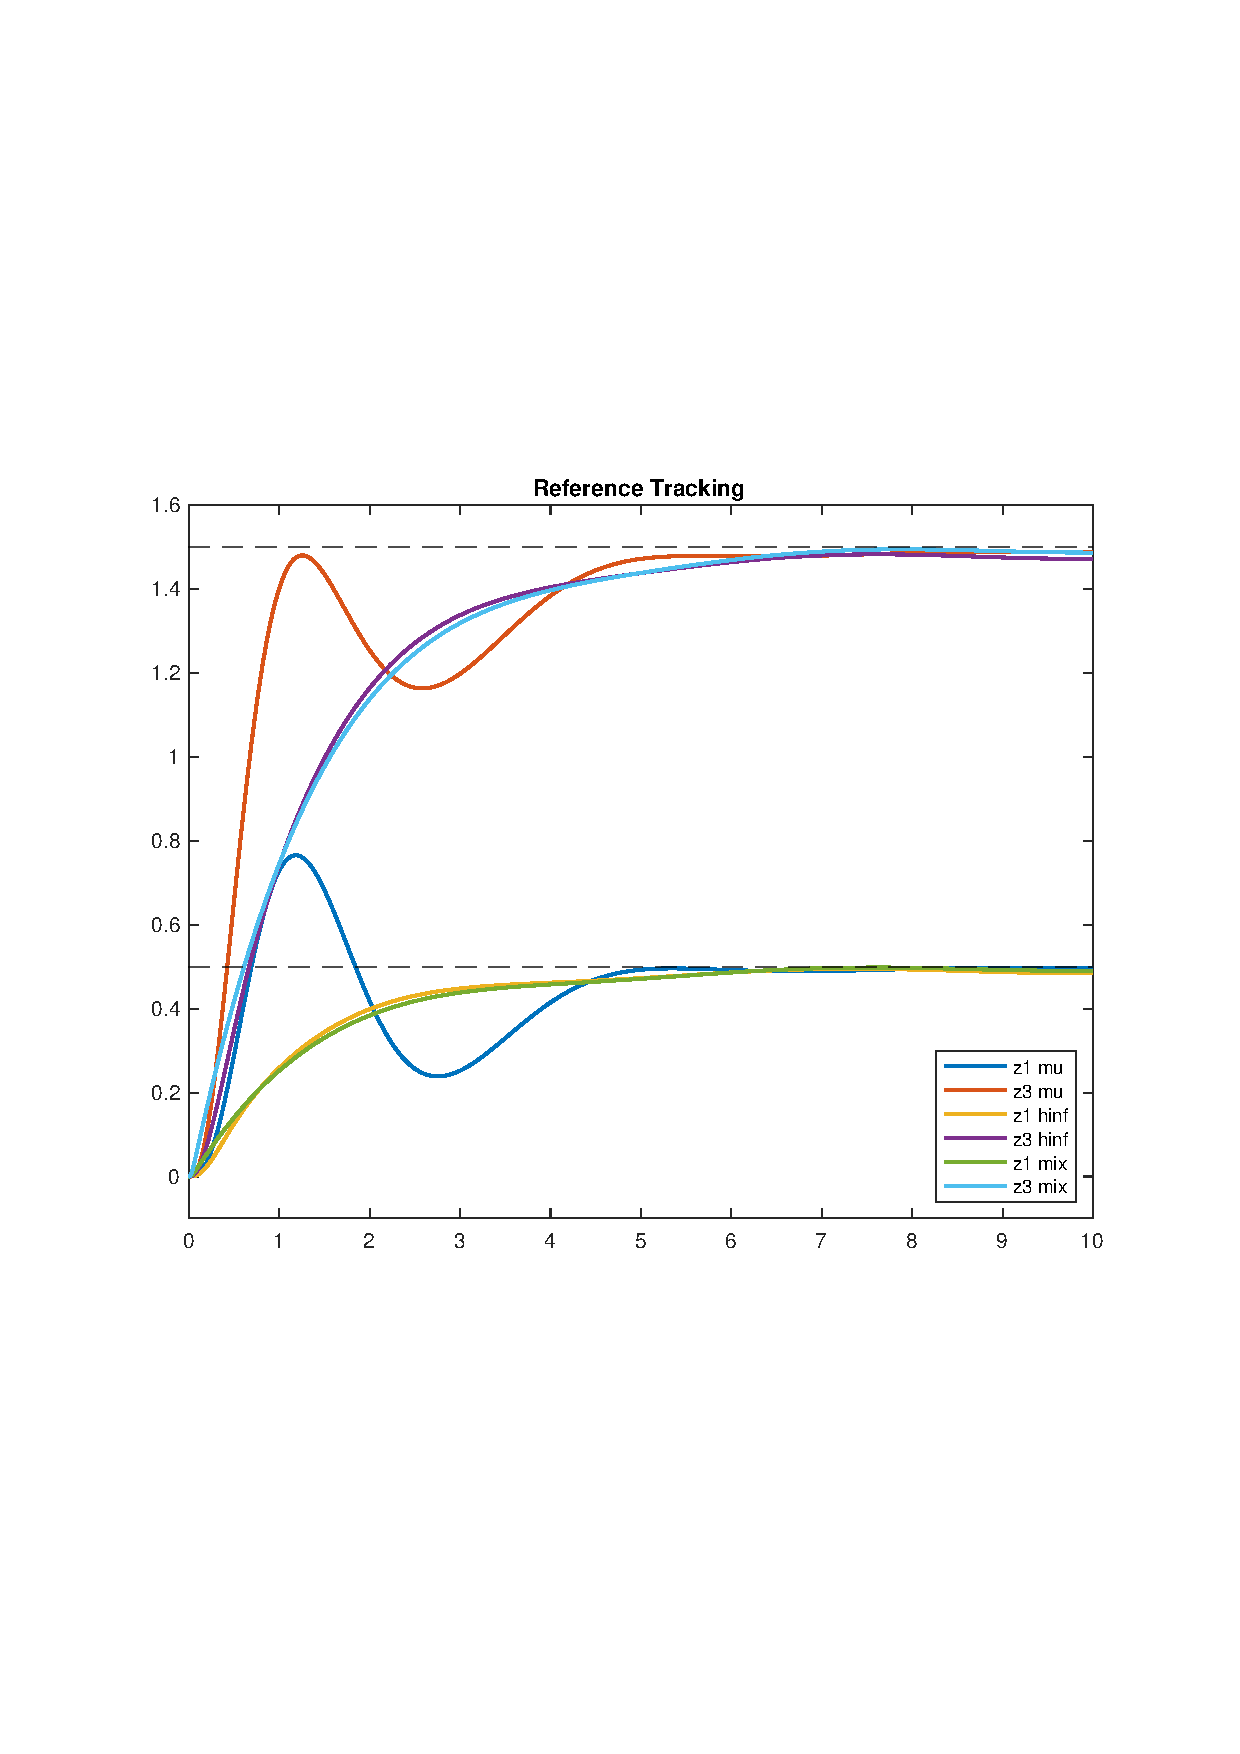
\includegraphics[width=\textwidth]{Figures/fig12a.pdf}}

\def\FigureTwelveB{\centering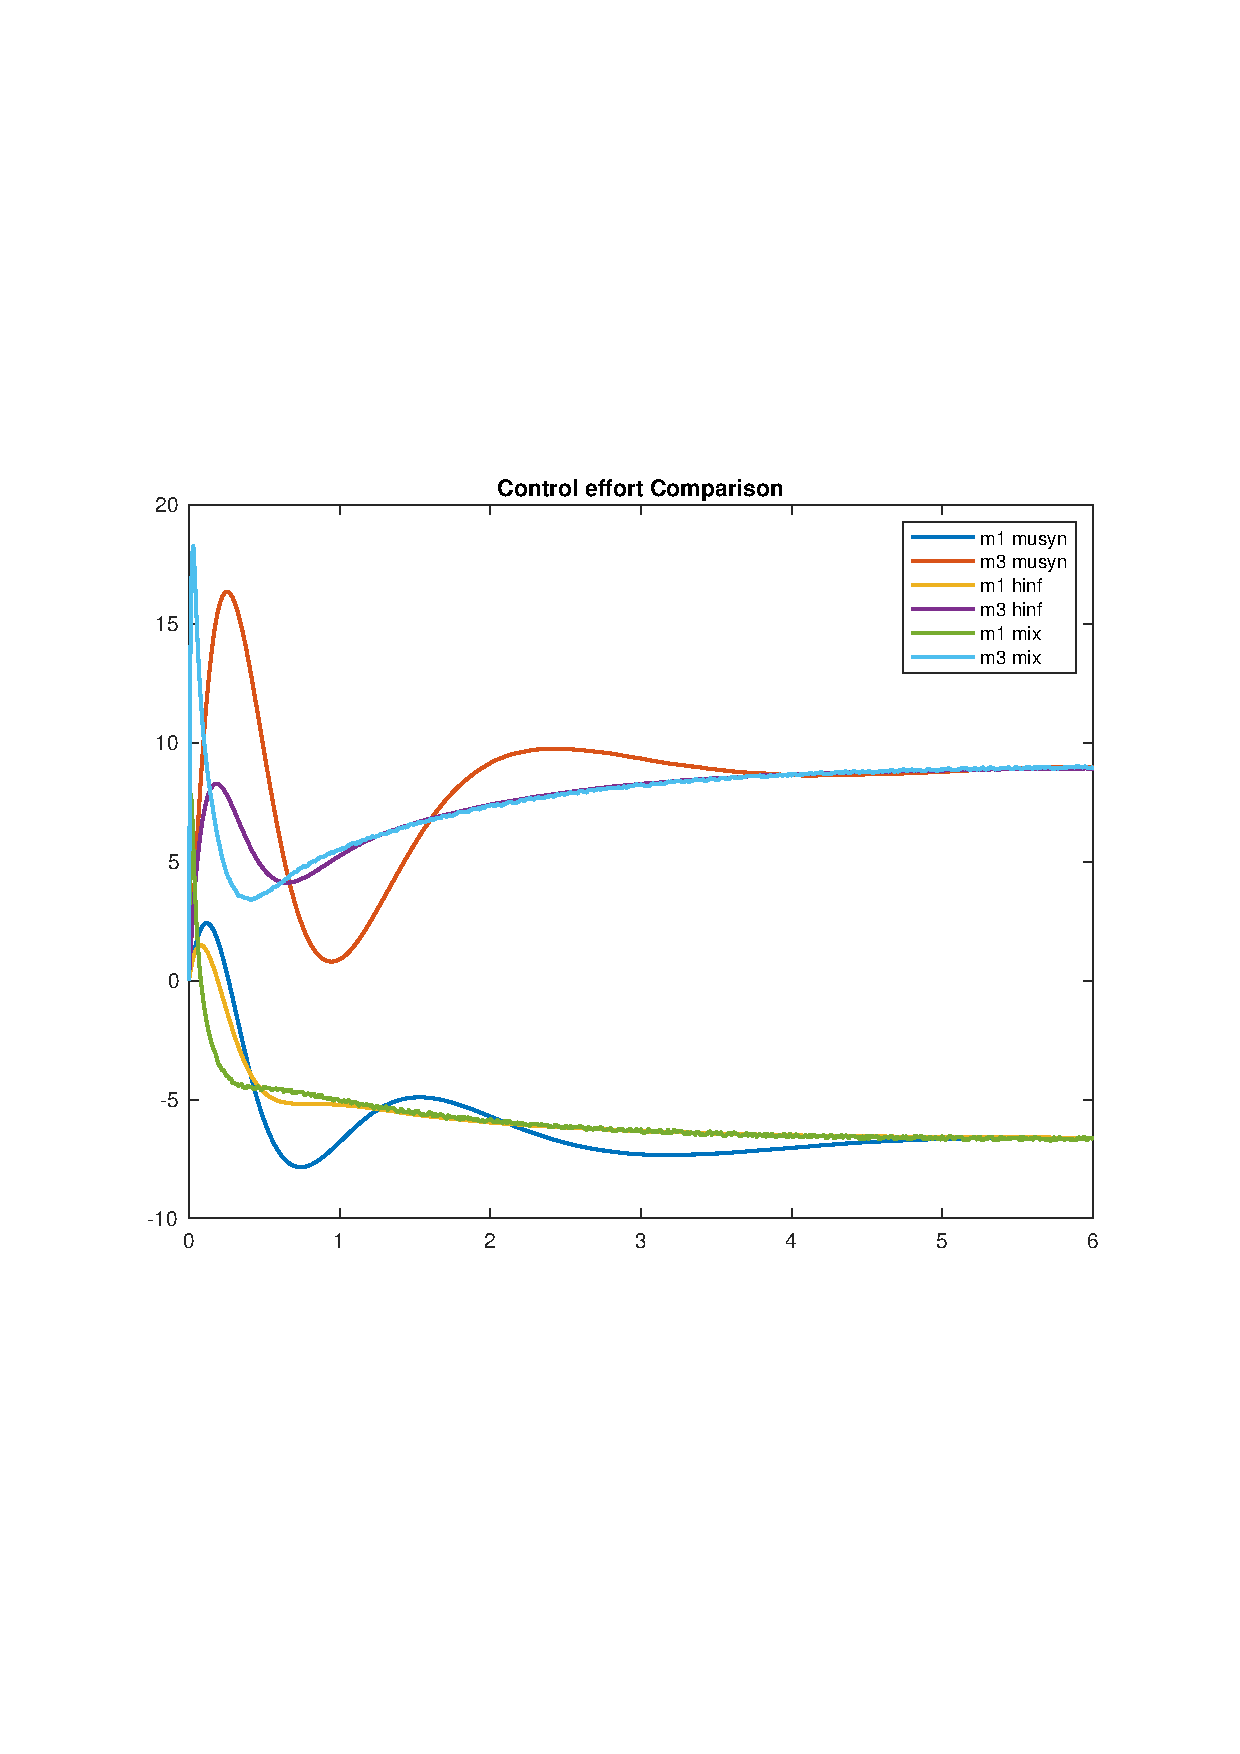
\includegraphics[width=\textwidth]{Figures/fig12b.pdf}}

\def\FigureTwelveC{\centering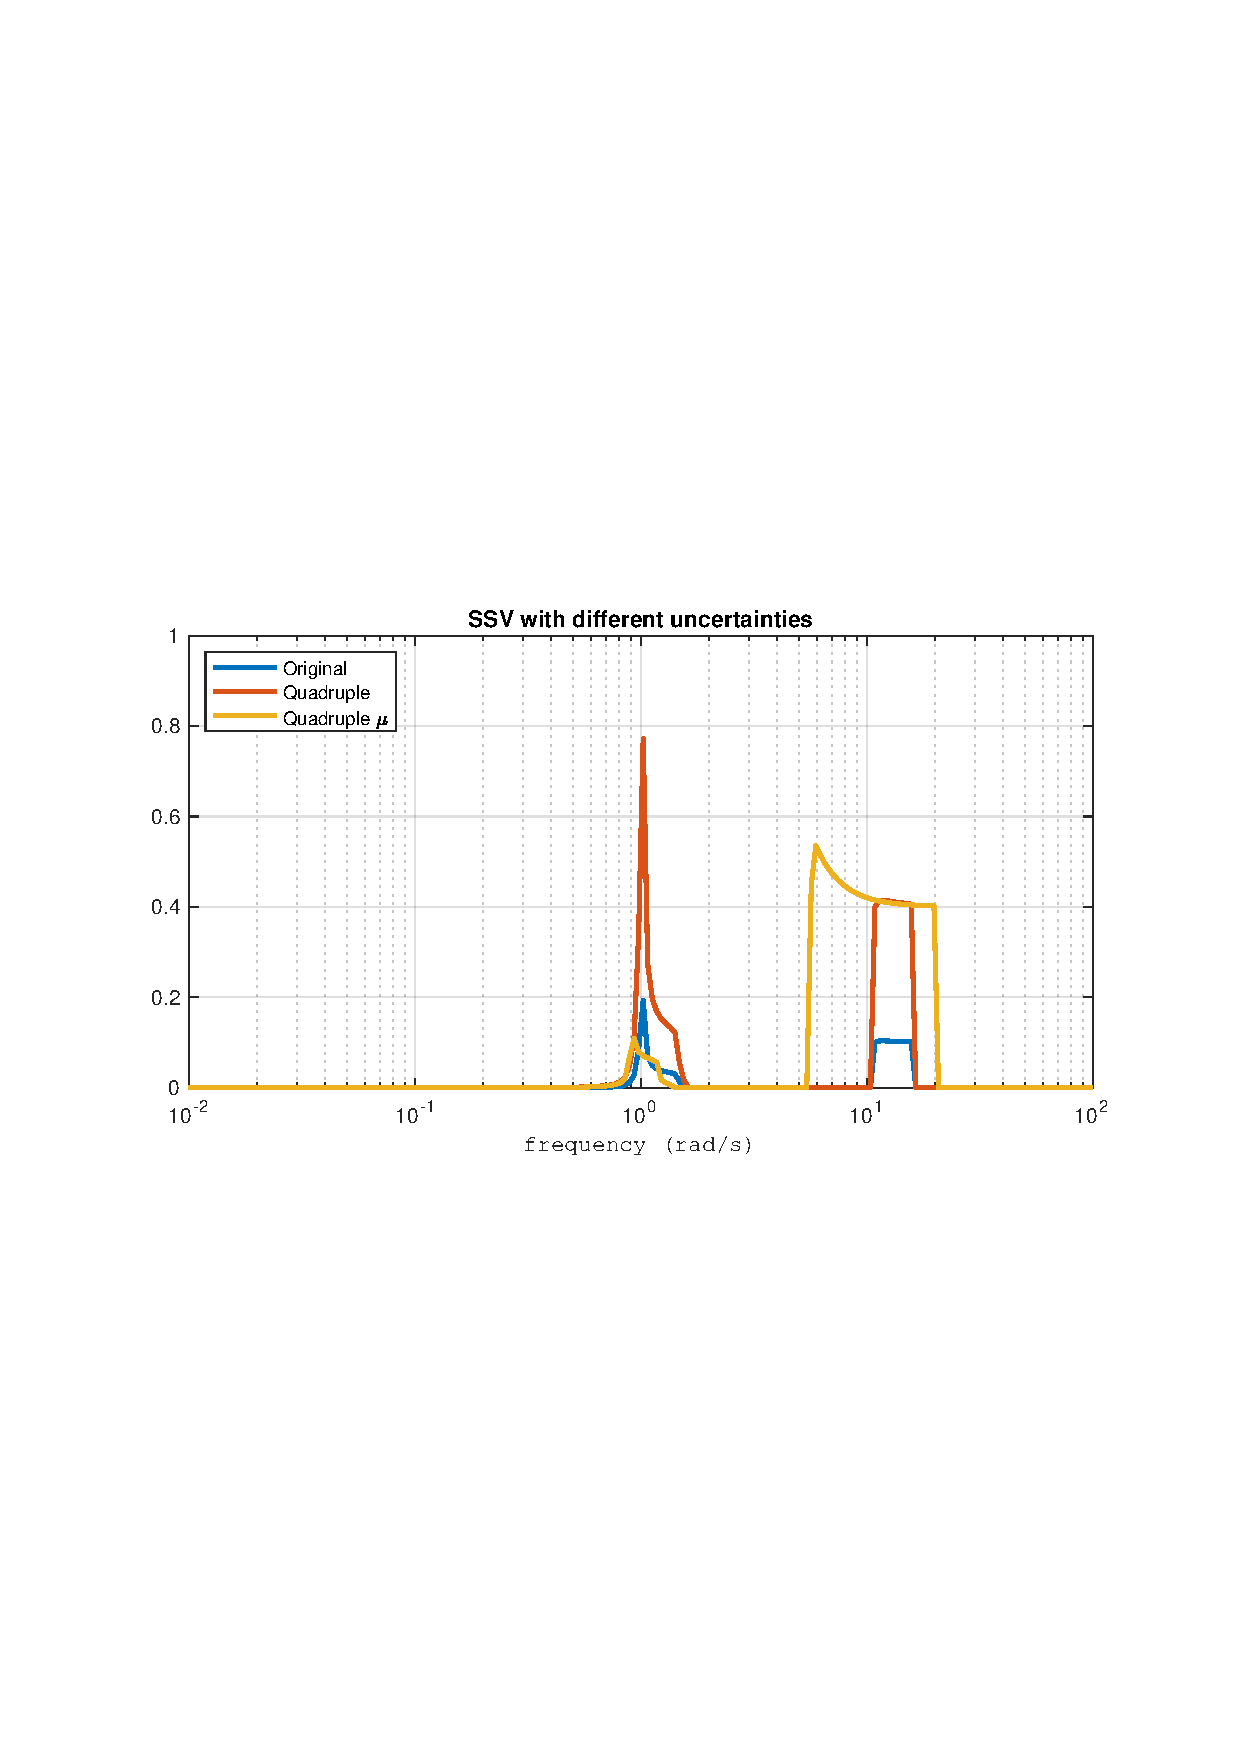
\includegraphics[width=\textwidth]{Figures/fig12c.pdf}}

\title{Multivariable Feedback Control \\ Homework 03}
\author{Matteo Scuderi\\ matricola 1937090}
\date{}

\begin{document}

\maketitle

\section{Problem 1: SVD for Augmented SISO systems}
In this first problem I consider a simple plant transfer function:
\begin{equation}
        G(s) = \frac{1}{s+10}
\label{eq:Model}
\end{equation}
I'll interpret its steady state behavior using augmented plants and their Singular Value Decomposition. The general control scheme is reported below (Fig.~\ref{fig:fig01}).
\begin{figure}[h!]
    \FigureOne
    \caption{General control scheme for Problem 1}
    \label{fig:fig01}
\end{figure}
\subsection{Spec1:$W_{1}(0)$ Gain}
The goal of this section is to find a controller $C_1(s)$ that ensure asymptotic tracking of constant references and use the augmented Plant to analyze the $W_{1}(0)$ gain's SVD. 
\\\\
We consider as inputs $(r, d_1, d_2)$ -respectively the reference, input and output disturbances- and as outputs the the tracking error and the control effort $(e_y, m)$.
\\\\
\textbf{Assuming} constant disturbances $d_1, d_2$, we can define our controller as a simple $C_1(s):= \frac{K}{s}$ - with a personal choice of $K = 10$ - to guarantee both astatism and exact asymptotic tracking.
\\\\
The resulting augmented plant is shown in Fig.~\ref{fig:fig02}:  
\begin{figure}[h!]
    \FigureTwo
    \caption{Augmented Plant for $(r,d_1,d_2)\longrightarrow(e_y,m)$}
    \label{fig:fig02}
\end{figure}
\\For this scheme, we can express all input-output relationships at closed loop as:
\begin{equation}
\begin{bmatrix}
e_y \\
m
\end{bmatrix}
=
\begin{bmatrix}
\frac{1}{1+GC_1} & -\frac{G}{1+GC_1} & -\frac{1}{1+GC_1} \\
\\
\frac{C}{1+GC_1} & -\frac{CG}{1+GC_1} & -\frac{C}{1+GC_1}
\end{bmatrix}
\begin{bmatrix}
r \\
d_1 \\
d_2
\end{bmatrix}
\label{eq:AugmentedPlant1}
\end{equation}
Calling the input-output matrix $W_1(s)$, we can finally compute the $W_1(j\omega)$ dc-gain and its Singular Value Decomposition for $\omega = 0$.
\subsubsection{SVD for $W_1(0)$}
The singular value decomposition comes as:
\begin{equation}
\begin{split}
        W_1(0) = 
\begin{bmatrix}
0 & 0 & 0 \\
10 & -1 & 10
\end{bmatrix} \qquad with: W_1(0) = U \Sigma V^T\\
        U = 
\begin{bmatrix}
0 & -1\\
1 & 0
\end{bmatrix},
        \Sigma = 
\begin{bmatrix}
14.1774 & 0 & 0 \\
0 & 0 & 0
\end{bmatrix},
        V = 
\begin{bmatrix}
0.7053 & -0.7089 & 0\\
-0.0705 & -0.0702 & -0.9950 \\  
 -0.7053 & -0.7018 & 0.0995
\end{bmatrix}
\end{split}
\label{eq:SVD-1}
\end{equation}
Notice that:
\begin{itemize}
\item \textbf{$rank( \Sigma )=1$}: The only singular value is $\sigma = 14.1774$ (since in reality it is a SISO system which has been "augmented")
\item $\mathcal{N}(W_1(0)):= gen\{(-0.7089\ -0.0702\ -0.7018)^T,
(0\ -0.9950\ 0.0995)^T\}$\\
\\Which means that \textbf{any linear combination of these two input directions correspond to a null output} $e_y=0; m=0$ \textbf{at steady state}. Therefore $\alpha v_1" + \beta v_2" = [0,0]^T\ \forall \alpha, \beta$. In particular, the second generator $v_{2}"$ shows that, zeroing out the reference $r=0$, the two disturbances totally compensate each other whenever $d_1 = -10d_2$.
\item $\mathcal{N}(W_1^T(0)):= gen\{(-1\ 0)^T\}$
\\ \\
From this we understand that any linear combination on this output direction gives zero as result. Therefore we have that $-\alpha e_y (+\ 0\ m) = 0$. This means that, regardless of the value of $m$,  \textbf{$e_y$ will always be zero}, which is coherent with our specifics on astatism and type one.
\item Since $u_1 = (0\ 1)$, we have that \textbf{the maximum amplification} will come along the $v_1' =(0.7053\ -0.0705\ -0.7053)$ input direction and will be exactly $\sigma$ in module, i.e. it will be affecting only the control effort. 
\end{itemize}
Some plots are reported in Fig.~\ref{fig:fig03}  , to show that the claims above have real counterpart in simulation.
\begin{figure}[h!]{}
    \begin{subfigure}[t]{0.32\textwidth}
           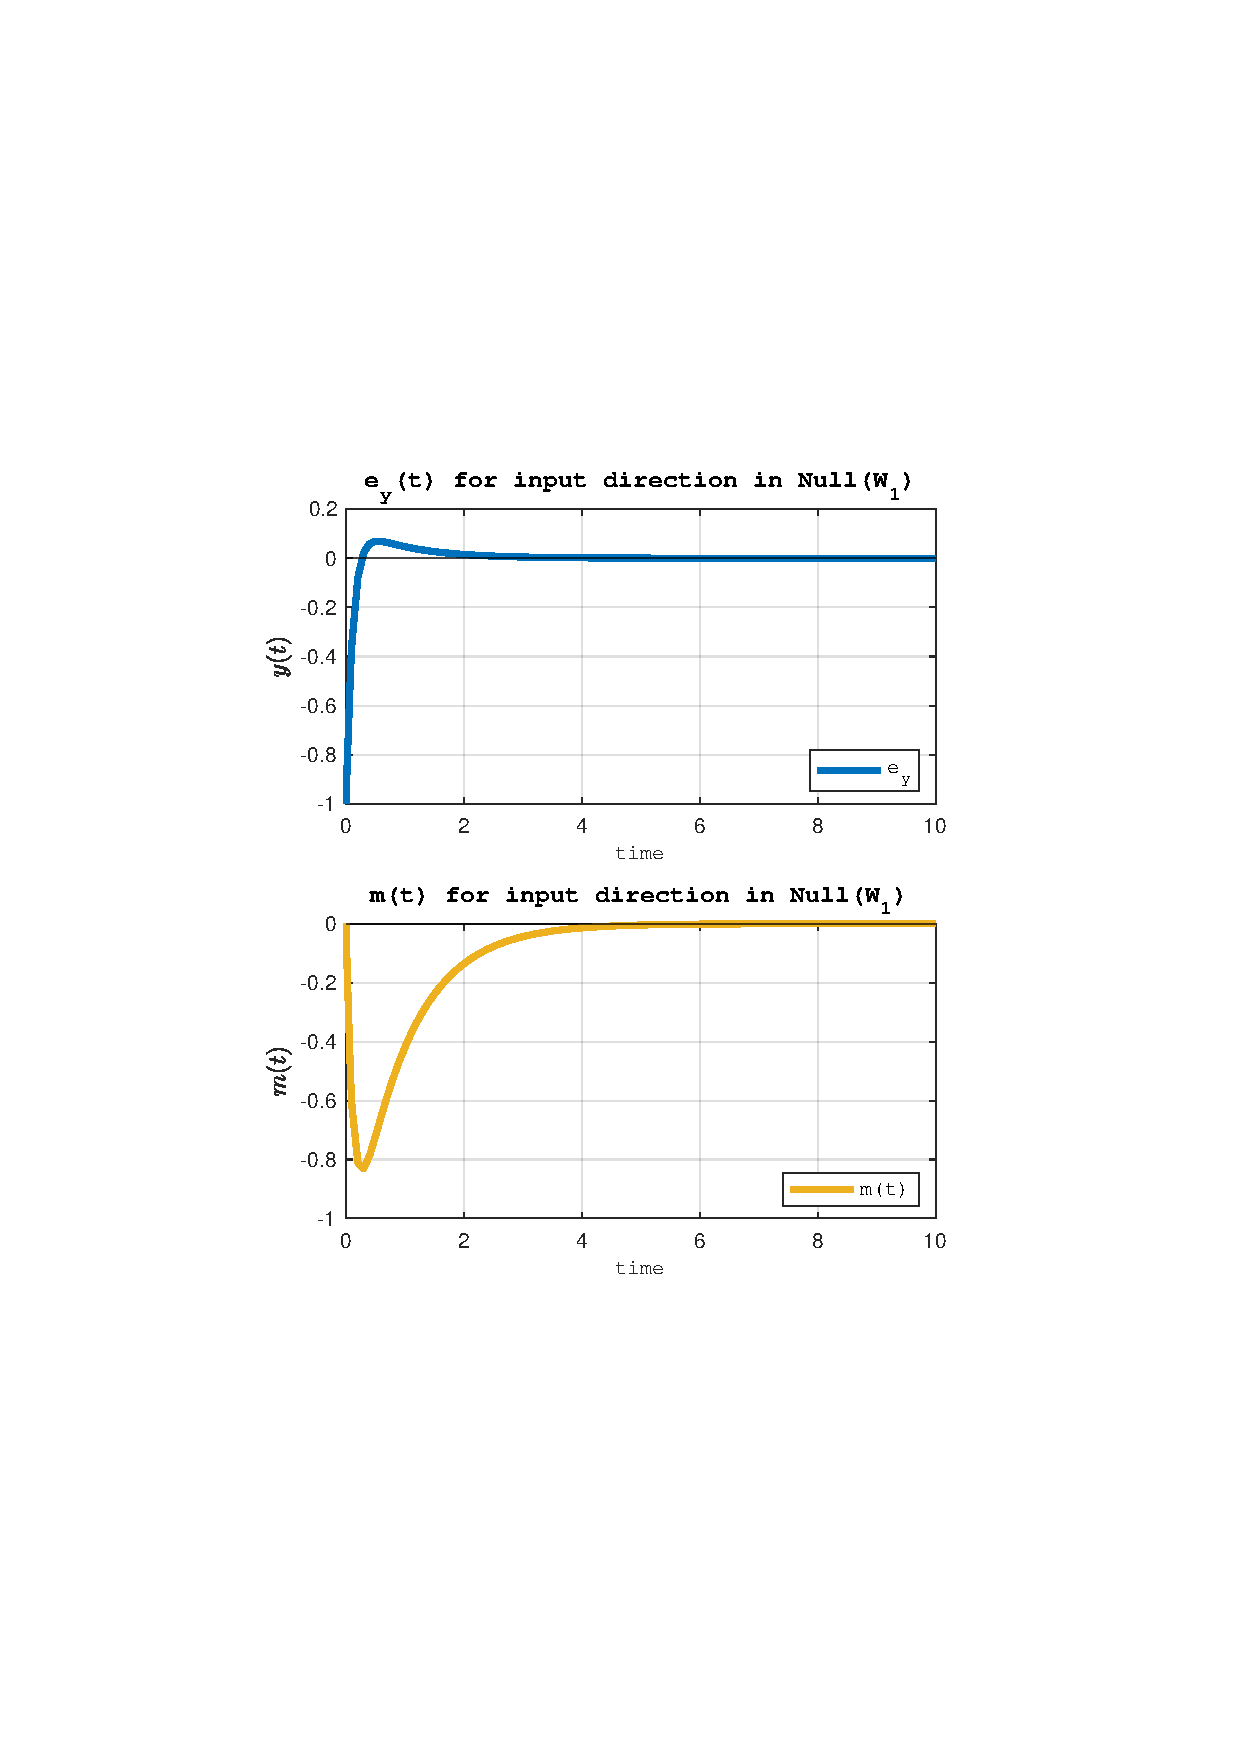
\includegraphics[width=\textwidth]{Figures/fig03a.pdf}
           \subcaption{Zero Output for $u =$\\$(0,-10, 1)^T\in\mathcal{N}(W_1(0))$}
           \label{fig:fig03a}
    \end{subfigure}
    \begin{subfigure}[t]{0.32\textwidth}
           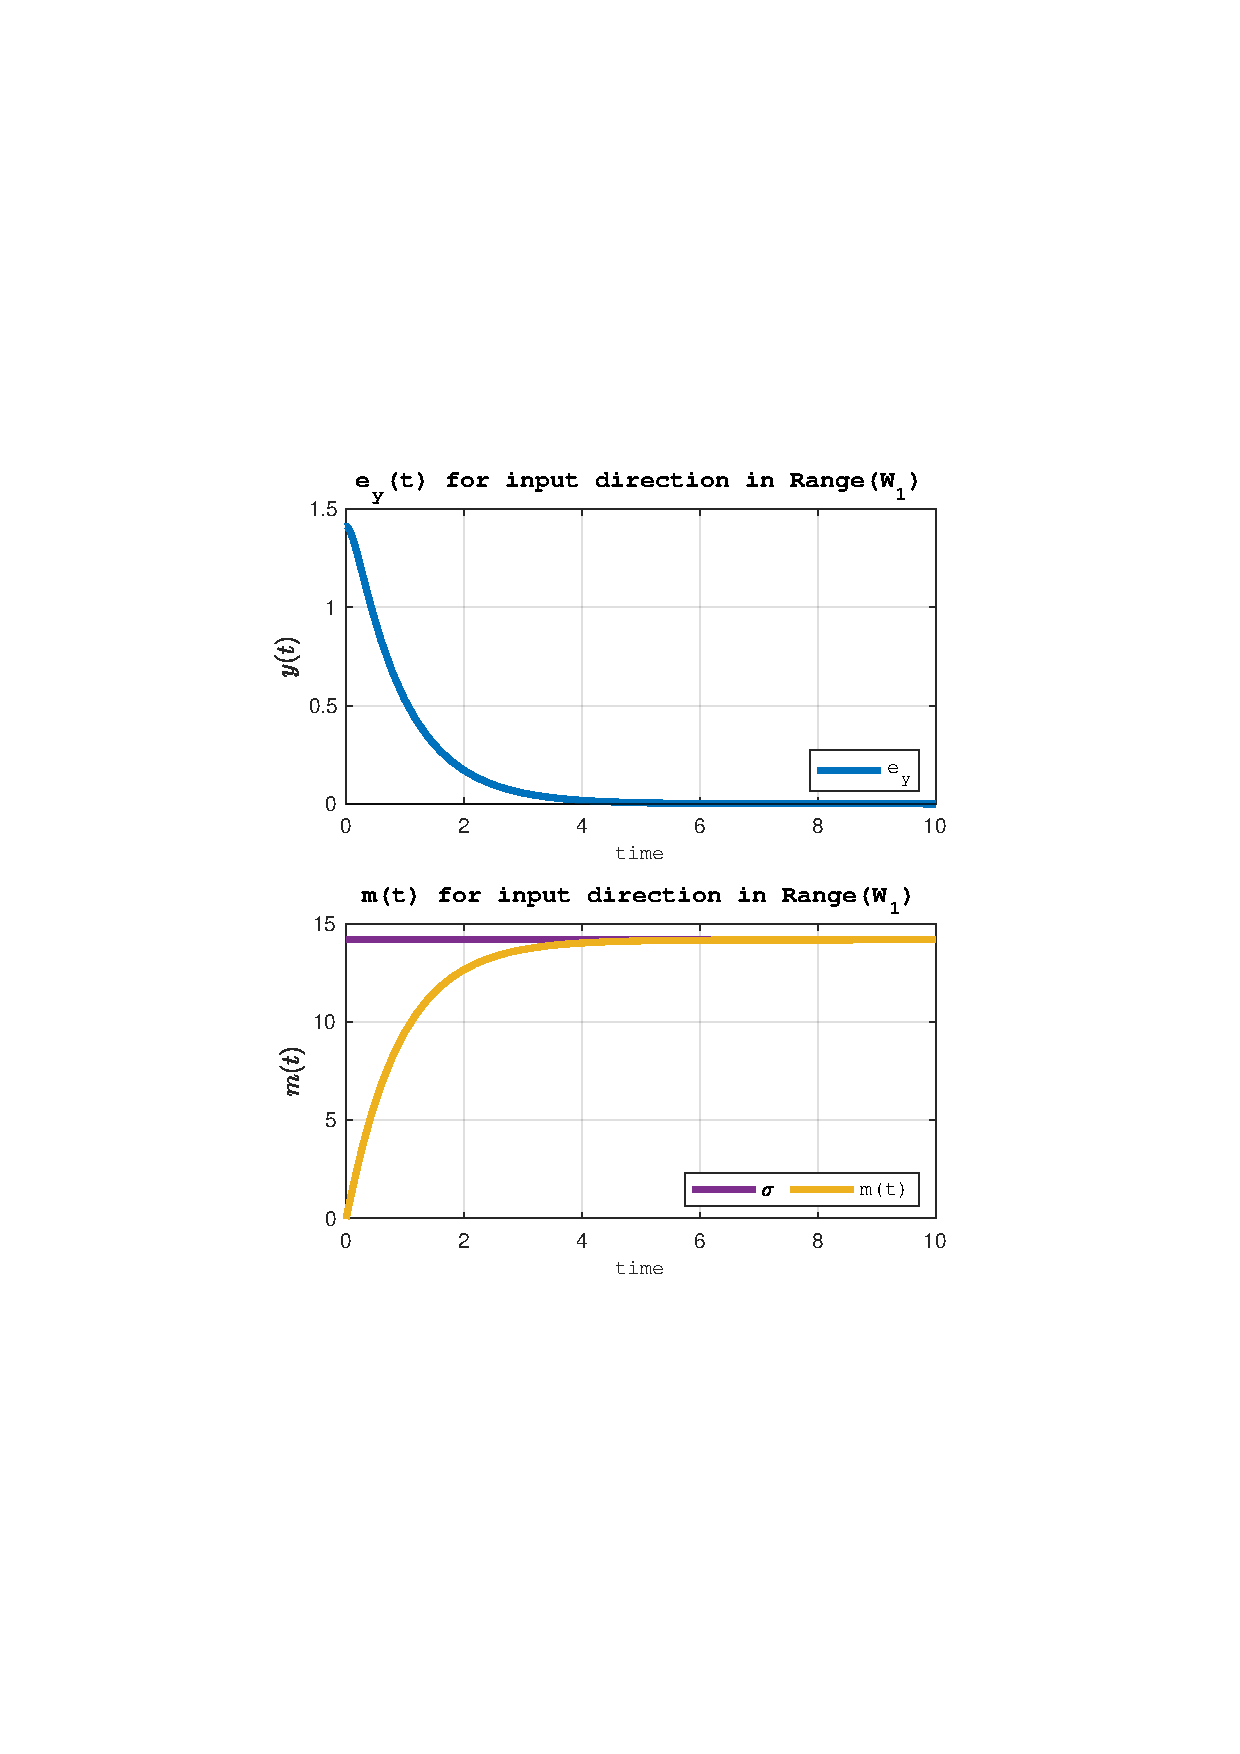
\includegraphics[width=\textwidth]{Figures/fig03b.pdf}
           \subcaption{Maximum $m$ \\amplification for $u=$\\ $(0.7053,-0.0705,-0.7053)^T \\ \in\mathcal{R}(W_1(0))$}
           \label{fig:fig03b}
    \end{subfigure}
    \begin{subfigure}[t]{0.32\textwidth}
           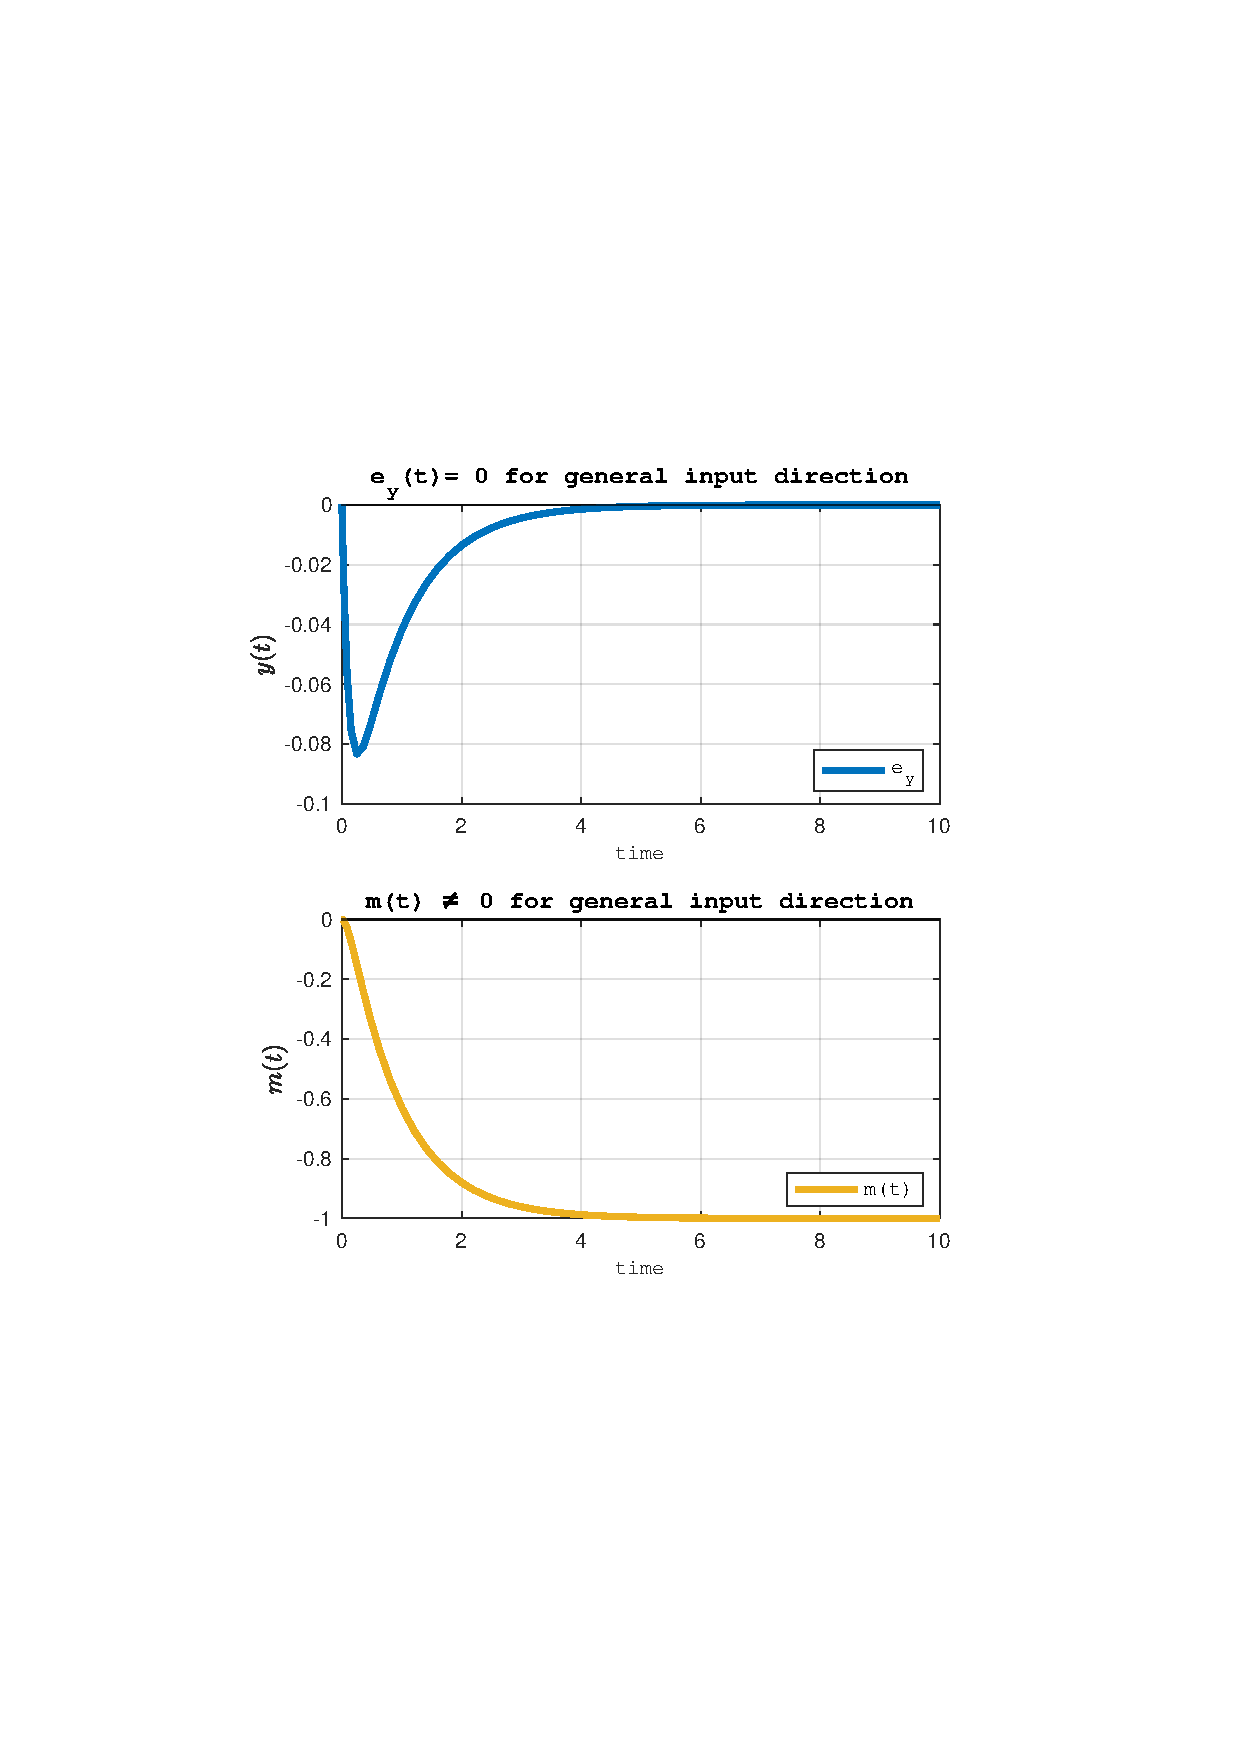
\includegraphics[width=\textwidth]{Figures/fig03c.pdf}
           \subcaption{Any input direction gives $e_y(t) = 0$ [from $\mathcal{N}(W_1^T(0)$)]}
           \label{fig:fig03c}
    \end{subfigure}
    \caption{Responses along different input direction}
    \label{fig:fig03}
   \end{figure}
\subsubsection*{Remark: Benefits of Augmented Plant}
As some results are intuitive and come from SISO system's theory, such as astatism and exact tracking, some others are not so noticeable for SISO systems. For example, from the study of $\mathcal{N}(W_1(0))$ we discovered the proportional relation between input and output disturbance, in order for them to compensate each other and annihilate control effort as well. Moreover, we found the input direction under which we have maximum control effort.

\subsection{Spec2: $W_{2}(\omega)$ Gain, $\omega=10$}
We now zero-out the disturbances $d_1,\ d_2$ and consider instead the augmented plant $W_2(s)$ with the measurement noise $n(t)$ as second input. The resulting scheme is shown below (Fig.~\ref{fig:fig04}).
\begin{figure}[h!]
    \FigureFour
    \caption{Augmented Plant for $(r,m)\longrightarrow(e_y,m)$}
    \label{fig:fig04}
\end{figure}
From here, we can express all input-output relations as:
\begin{equation}
\begin{bmatrix}
y \\
m
\end{bmatrix}
=
\begin{bmatrix}
\frac{GC_2}{1+GC_2} & -\frac{GC_2}{1+GC_2} \\
\\
\frac{C_2}{1+GC_2} & -\frac{C_2}{1+GC_2}
\end{bmatrix}
\begin{bmatrix}
r \\
n
\end{bmatrix}
\label{eq:AugmentedPlant2}
\end{equation}
\subsubsection*{Remark: Preliminary considerations}
\begin{itemize}
\item The chosen controller $C_2(s)$ has been designed via $H_\infty$ control for the SISO system. The control paradigm was: increasing bandwidth for properly tracking the reference, but do not push it too high for maintaining some level of noise rejection. The exact sensitivity weights can be found in the Matlab file.
\item Measurement noise usually has an higher frequency content than the reference's ($\omega = 10$). Therefore, for the moment we consider a simplified noise  $\Tilde{n}(t) = M_nsin(10t+\Phi_n)$ to highlight the properties found when using the SVD.
\end{itemize}
\subsubsection{SVD for $W_2(j\omega),\ \omega=10$}
From the singular value decompositions we get once again that the $\Sigma$ matrix is not full rank and the only singular value is $\sigma= 19.4589$. 
The complex directions $v_i,\ u_i$ analysis leads to the following results:\\\\
\textbf{Maximum Amplification:} \\We have that the following "complex input direction"
\begin{equation*}
\begin{bmatrix}
r_{max}(t) \\ n_{max}(t)
\end{bmatrix} =
\begin{bmatrix}|v_{11}|\sin(\Bar{\omega}  t + \angle v_{11}) \\ |v_{12}|\sin(\Bar{\omega}  t + \angle v_{12}) \end{bmatrix} =
\begin{bmatrix}
(\sqrt{2}/2)sin(10 t+\pi) \\
(\sqrt{2}/2)sin(10 t)
\end{bmatrix}
\end{equation*}
gives maximum amplification in the form of the outputs:
\begin{equation*}
\begin{bmatrix}
y_{max}(t) \\ m_{max}(t)
\end{bmatrix} =
\begin{bmatrix}\sigma|u_{11}|\sin(\Bar{\omega}  t + \angle u_{11}) \\ |u_{12}|\sin(\Bar{\omega}  t + \angle u_{12}) \end{bmatrix} =
\begin{bmatrix}
(1.3725)sin(10 t + 3.0224) \\
(19.4104)sin(10 t -2.4754)
\end{bmatrix}
\end{equation*}
Therefore we find out that we have \textbf{maximum amplification} whenever the reference and the noise have \textbf{same amplitude} (very bad noise) and a phase of 180° w.r.t. each other) - see Fig.~\ref{fig:fig05} -\\\\
\textbf{Null Output:} \\We have that the input signals cancel out each other and give zero output whenever reference and noise exactly coincide in magnitude and phase ($r(t) = n(t)$, not at all realistic).

\subsubsection*{Remark: Validity of the results}
Notice however -as previously mentioned- that in reality, these extreme cases are never actually met, since the noise acts at higher frequency than $\omega = 10$. Moreover, noise has usually a smaller magnitude than the reference, up to two or three orders of magnitude lower. Therefore, the input directions considered with the SVD are useful in terms of understanding the theory, but unrealistic in practice.
\begin{figure}[h!]
    \FigureFive
    \caption{Maximum output amplification}
    \label{fig:fig05}
\end{figure}

\clearpage
\section{Problem 2: Importance of Scaling 2x2 MIMO system}
Let's consider a Mass-Spring-Damper system that has two energy sources: a towing force "externally" applied  (we can think of a cable attached to a winch) and a DC motor on the front wheel of the chart.\\
\\ Our \textbf{control inputs} will therefore be the DC motor armature Voltage $V(t)$ and the towing force generated by the winch $f(t)$.\\\\
We're interested in controlling the $x(t)$ position of the chart and make it reach a constant desired position, but we're also interested in the armature current $i(t)$, to guarantee that the motor operates safely. These two variables, of which we have direct measurements thanks to our sensors, will be out \textbf{system outputs} 
\begin{figure}[h!]
    \FigureSix
    \caption{MSD MIMO system }
    \label{fig:fig06}
\end{figure}
\subsection{Model Construction}
We can consider the state space representation of our 2x2 MIMO system to be defined by the matrices:
\begin{equation}
    \begin{bmatrix}
    \dot{x}_1 \\
    \dot{x}_2 \\
    \dot{x}_3 \\
    \end{bmatrix} =
    \begin{bmatrix}
    0 & 1 & 0 \\
    -\frac{k}{m} & -\frac{\mu}{m} & \frac{K_t}{mr} \\
    0 & -\frac{K_e}{L} & -\frac{R}{L}\\
    \end{bmatrix}
    \begin{bmatrix}
    x_1 \\
    x_2 \\
    x_3
    \end{bmatrix} +
    \begin{bmatrix}
    0 & 0\\
    0 & \frac{1}{m}\\
    \frac{1}{Lr} & 0\\
    \frac{1}{m_2}
    \end{bmatrix}
    \begin{bmatrix}
    u_1 \\ u_2  
    \end{bmatrix} 
    \quad \quad
    y = 
    \begin{bmatrix}
    x_1 \\ x_3  
    \end{bmatrix}
\end{equation}
with $x_1(t) := x(t)$ [position]; \quad $x_2(t) := v(t)$ [velocity]; \quad $x_3(t) := i(t)$ [armature current]; \quad $u_1(t) := V(t)$ [armature voltage]; \quad $u_2(t) := f(t)$ [winch force].
\\\\
From there, we can derive our MIMO 2x2 plant transfer function as:
\begin{equation}
        G(s) = 
    \begin{bmatrix}
        G_{11}(s) & G_{12}(s) \\ 
        G_{21}(s) & G_{22}(s)
    \end{bmatrix}\quad with\ each\ block\ being:
\end{equation}
\begin{align*}
    G_{11} = \frac{K_t/r^2}{(L m)s^3 + (L \mu + R m)s^2 + (K_e K_t / r + R \mu + L k)s + (R k )} \\
    G_{12} = \frac{R + Ls}{(L m)s^3 + (L \mu + R m)s^2 + (K_e K_t / r + R \mu + L k)s + (R k )} \\
    G_{21} = \frac{(ms^2 + \mu s + k)/r}{(L m)s^3 + (L \mu + R m)s^2 + (K_e K_t / r + R \mu + L k)s + (R k )} \\
    G_{22} = \frac{-K_e s}{(L m)s^3 + (L \mu + R m)s^2 + (K_e K_t / r + R \mu + L k)s + (R k )} \\
\end{align*}
\subsubsection{Remark: Condition Number}
Computing the $G(0)$ gain and its SVD we get that the two singular values are approximately $\Bar{\sigma} = 0.9685$ and $\underline{\sigma} = 0.0484$, leading to a large condition number of about $\kappa = 20$.
\\ This is a problem for both design and robust stability, since a small change in input directions could have huge effects in the output, even leading to instability. We'll therefore try to \textbf{mitigate this phenomenon using some proper scaling}.
\subsection{Formulation and Plant Scaling}
Let's now try to characterize the problem to justify the scaling and make it consistent.\\
\\First of all, the motor parameters are taken from \hyperlink{https://www.researchgate.net/publication/272102820_Parameters_Identification_of_a_Permanent_Magnet_DC_Motor}{this paper} and we derive that that:
\begin{itemize}
    \item The maximum armature voltage $V(t)$ is $V_{max} = \pm 3 V$
    \item The maximum armature current $i(t)$ is $i_{max} = \pm 3A$
    \item We have that the motor torque applied to the wheel is $\tau(t) = K_t i(t)$ and the traction force is then $MF = \tau / r$, with $r$ being the wheel radius. Picking $r = 0.35m$ (average wheel radius for a car) we can find the \textbf{maximum motor traction force} $MF_{max} = K_t i_{max} / r \approx 15.7 N$ 
\end{itemize}
Now, we've found out that the DC motor can supply a traction force non exceeding $15.7 N$.\\ However, assuming we want to reach a constant position $x_{des} = 1m$, we need to counter the spring elastic force $F_e = k x_{des} = 20N < MF_{max}$. \\It's clear that \textbf{the motor alone can't possibly "win" the elastic force at the desired position}.\\
That's why we have a supplementary source of traction force coming from the winch, which we assume able to supply up to $f_{max} = 15N$.
\\\\
The scaling weights are naturally defined from the bounds previously discussed: $w_V = 3;\ w_f = 15$. The scaled plant can be seen in the block diagram below.
\begin{figure}[h!]
    \FigureSeven
    \caption{Plant input Scaling}
    \label{fig:fig07}
\end{figure}
After properly scaling the plant, we can complete the augmented Plant scaling also with respect to the references and the tracking error.
\\The final control scheme for synthesis - adding performance weights - is:
\begin{figure*}[h!]
    \FigureAugmented
    \caption*{Augmented Plant with scaling for synthesis}
    \label{fig:aug_plant}
\end{figure*}
\\With $D_e \equiv D_r = \begin{bmatrix}
1 & 0 \\
0 & 2
\end{bmatrix}$; $R =  D_e^{-1}D_r = \begin{bmatrix}
1 & 0 \\
0 & 1
\end{bmatrix}$ and $w_S(s), w_U(s)$ sensitivity and control sensitivity weights.
\subsection{Simulation Results}
For the first time, despite numerous tries, I found some simulation results that are in clear contrast with what the theory suggests. 
\\\\
There must be some problem with the scaling I adopted, because it appears like it causes a decreases the performance instead of improving it.
\\\\
A more detailed description of my attempts can be found in the Matlab file "Problem2\_Scaling", while here I'll just sum up the obtained results.
\\\\
Trying to introduce scaling (in the form previously discussed) in the controller synthesis' scheme leads to poor performing controllers. Even removing some of the scaling matrices doesn't change the situation significantly. 
\\
One of the "best" performances obtained with scaling is about 6 times slower than the unscaled one. 
We can also notice a much more oscillating behavior in transient.
\begin{figure*}[h!]{}
    \begin{subfigure}[t]{0.45\textwidth}
    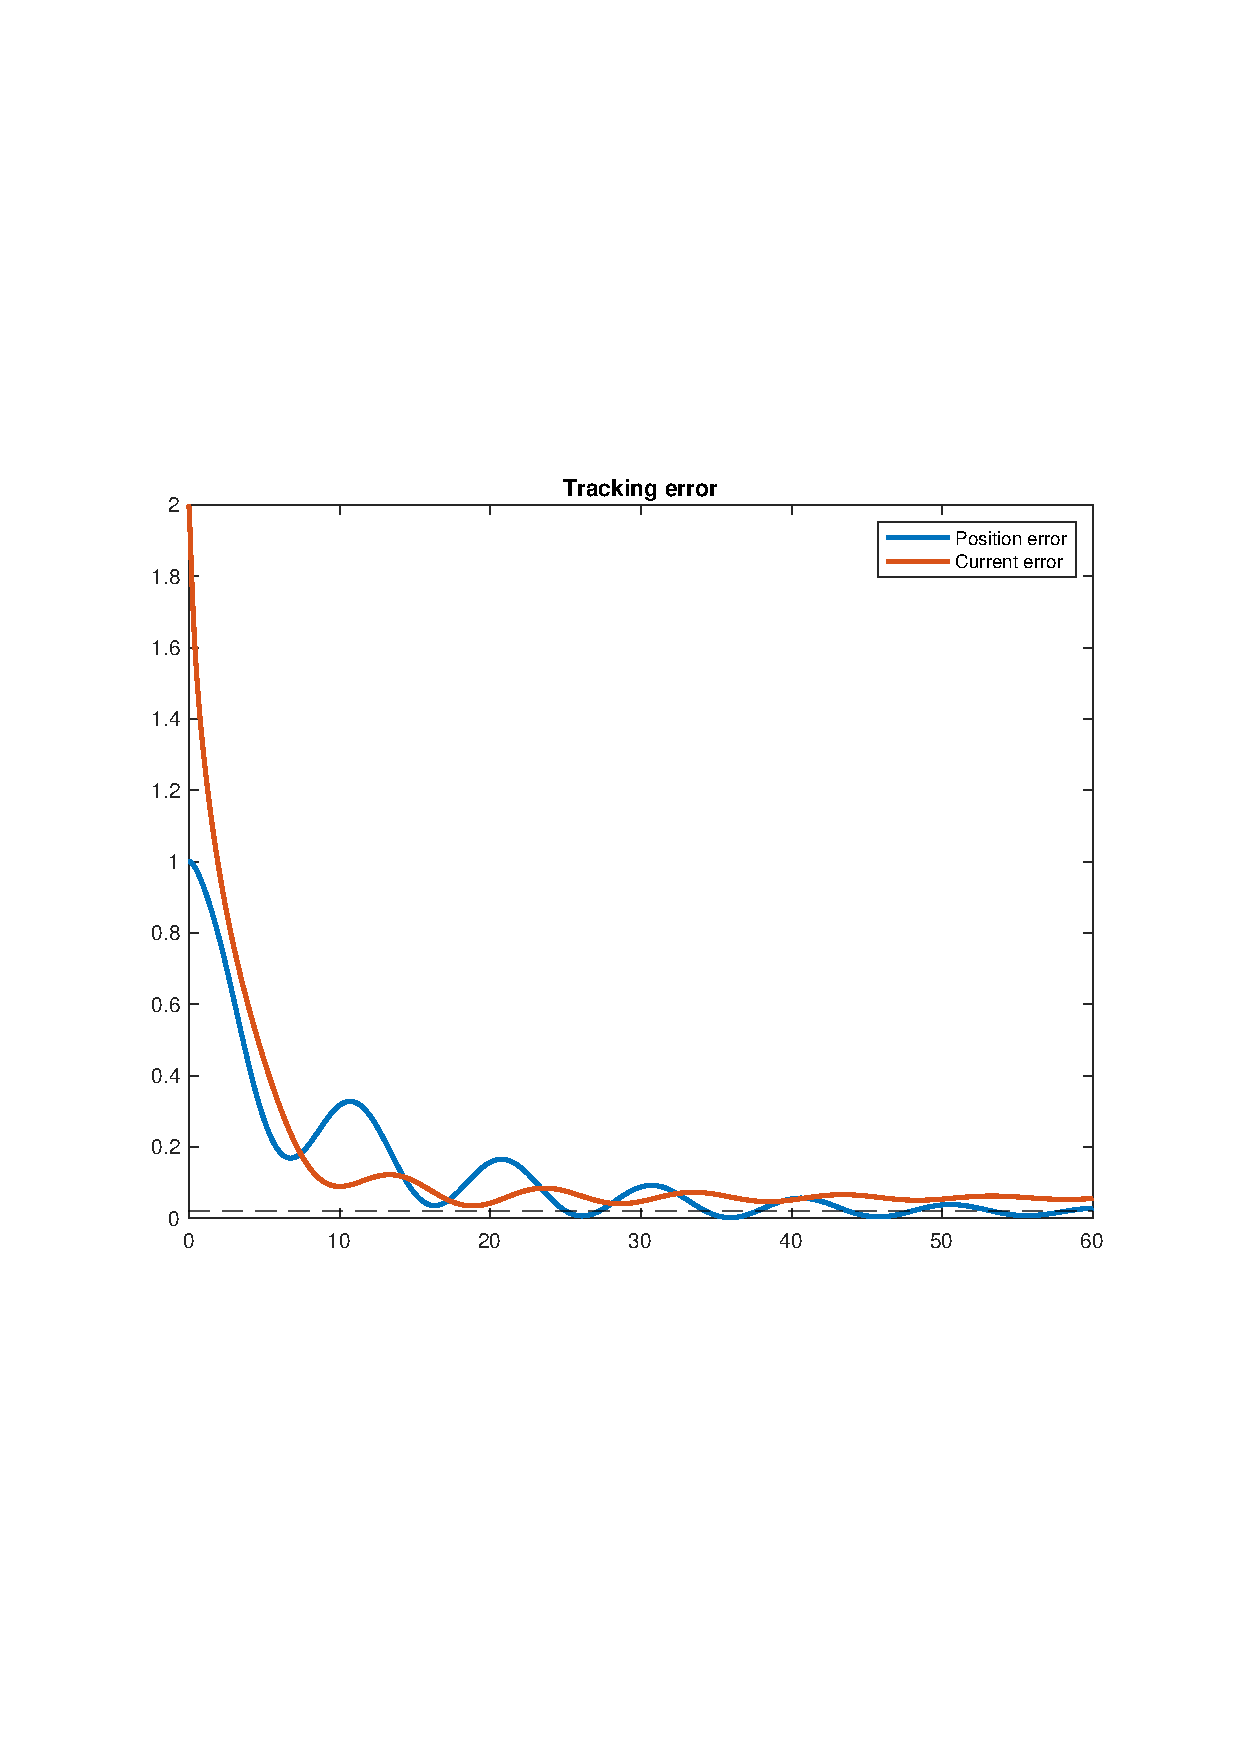
\includegraphics[width=\textwidth]{Figures/scaled.pdf}
           \subcaption*{Tracking Error: Scaled}
           \label{fig:scaled}
    \end{subfigure}
    \begin{subfigure}[t]{0.45\textwidth}
    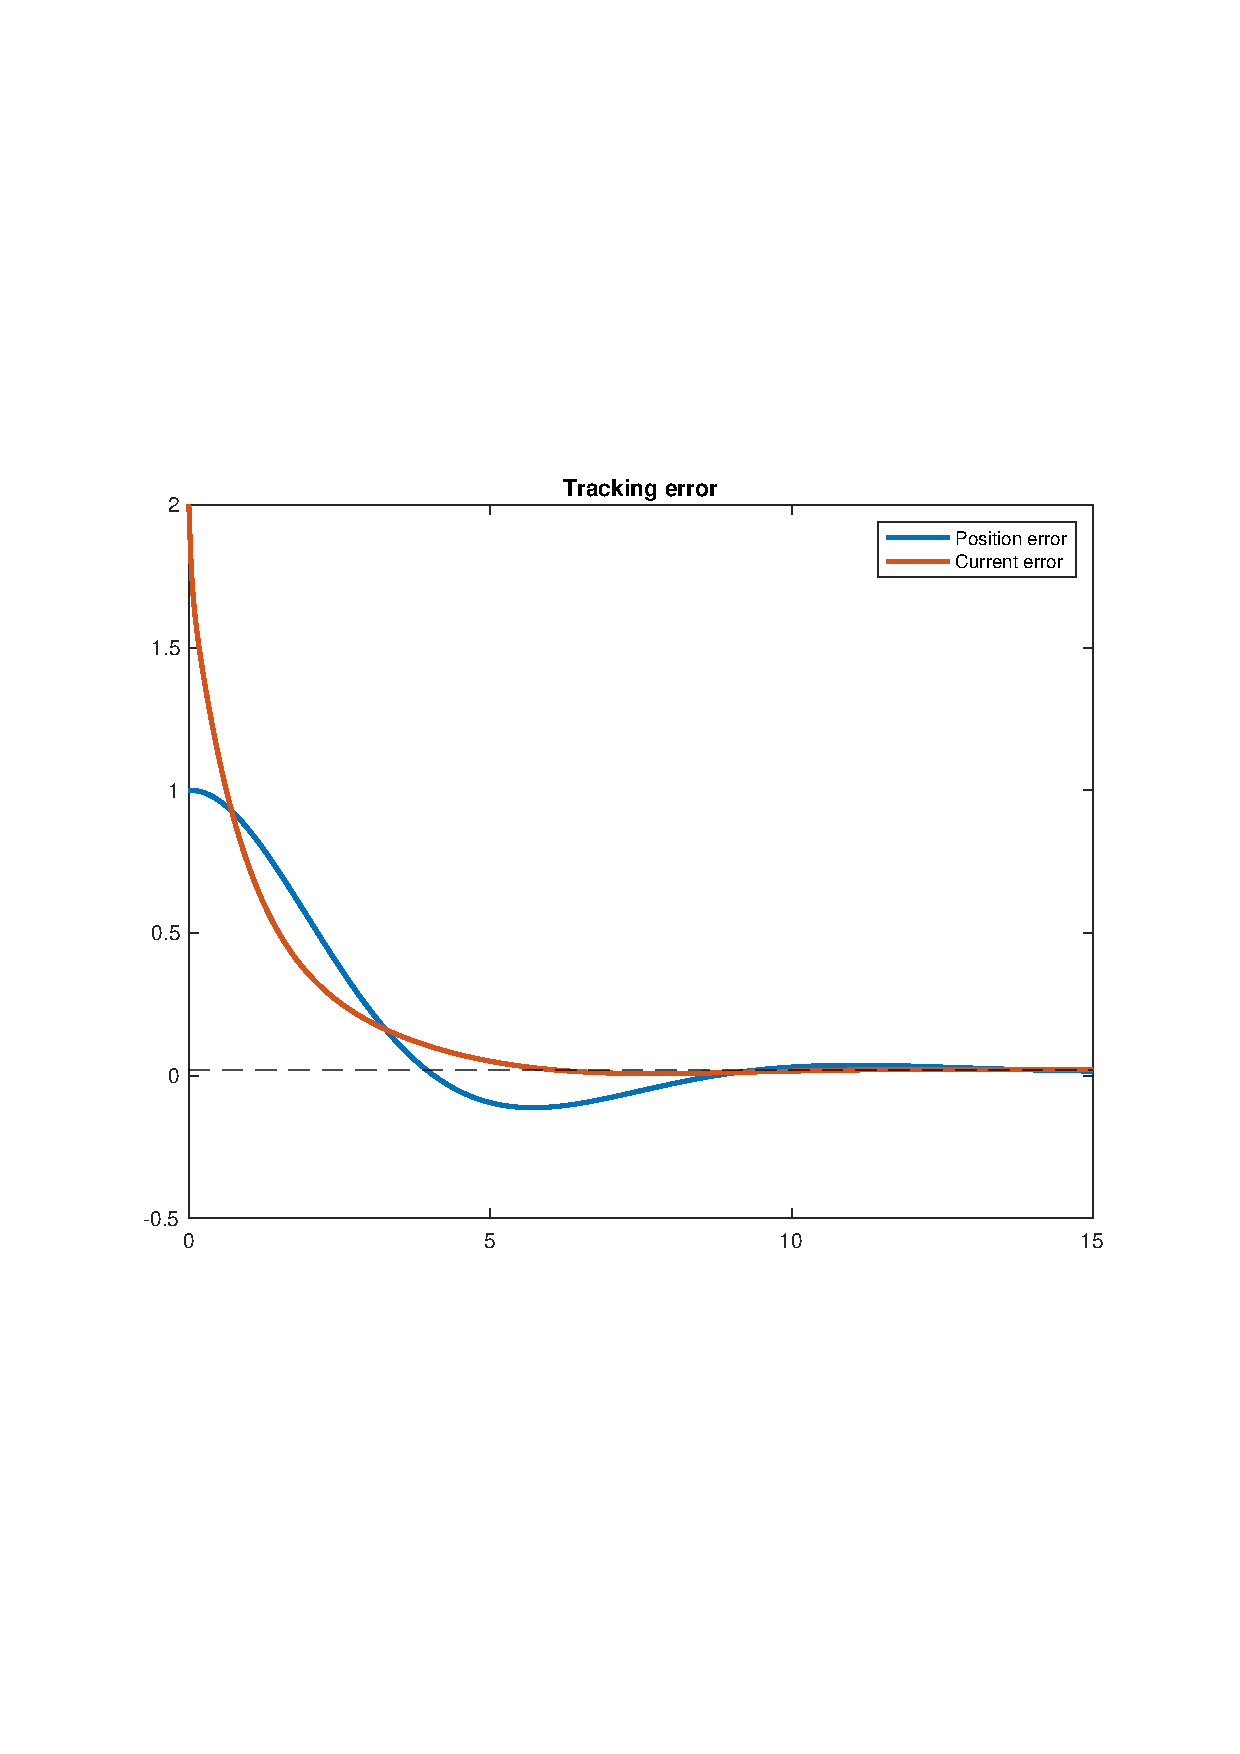
\includegraphics[width=\textwidth]{Figures/unscaled.pdf}
           \subcaption*{Tracking Error: Unscaled}
           \label{fig:unscaled}
    \end{subfigure}
    \caption*{Scaled vs Unscaled tracking error (notice also timescale)}
    \label{fig:unscaled}
   \end{figure*}
\clearpage
\section{Problem 3: MIMO Robust stability}
It this section we study robust stability, using a triple MSD system with two force inputs $f_1,\ f_3$.
\begin{figure*}[h!]
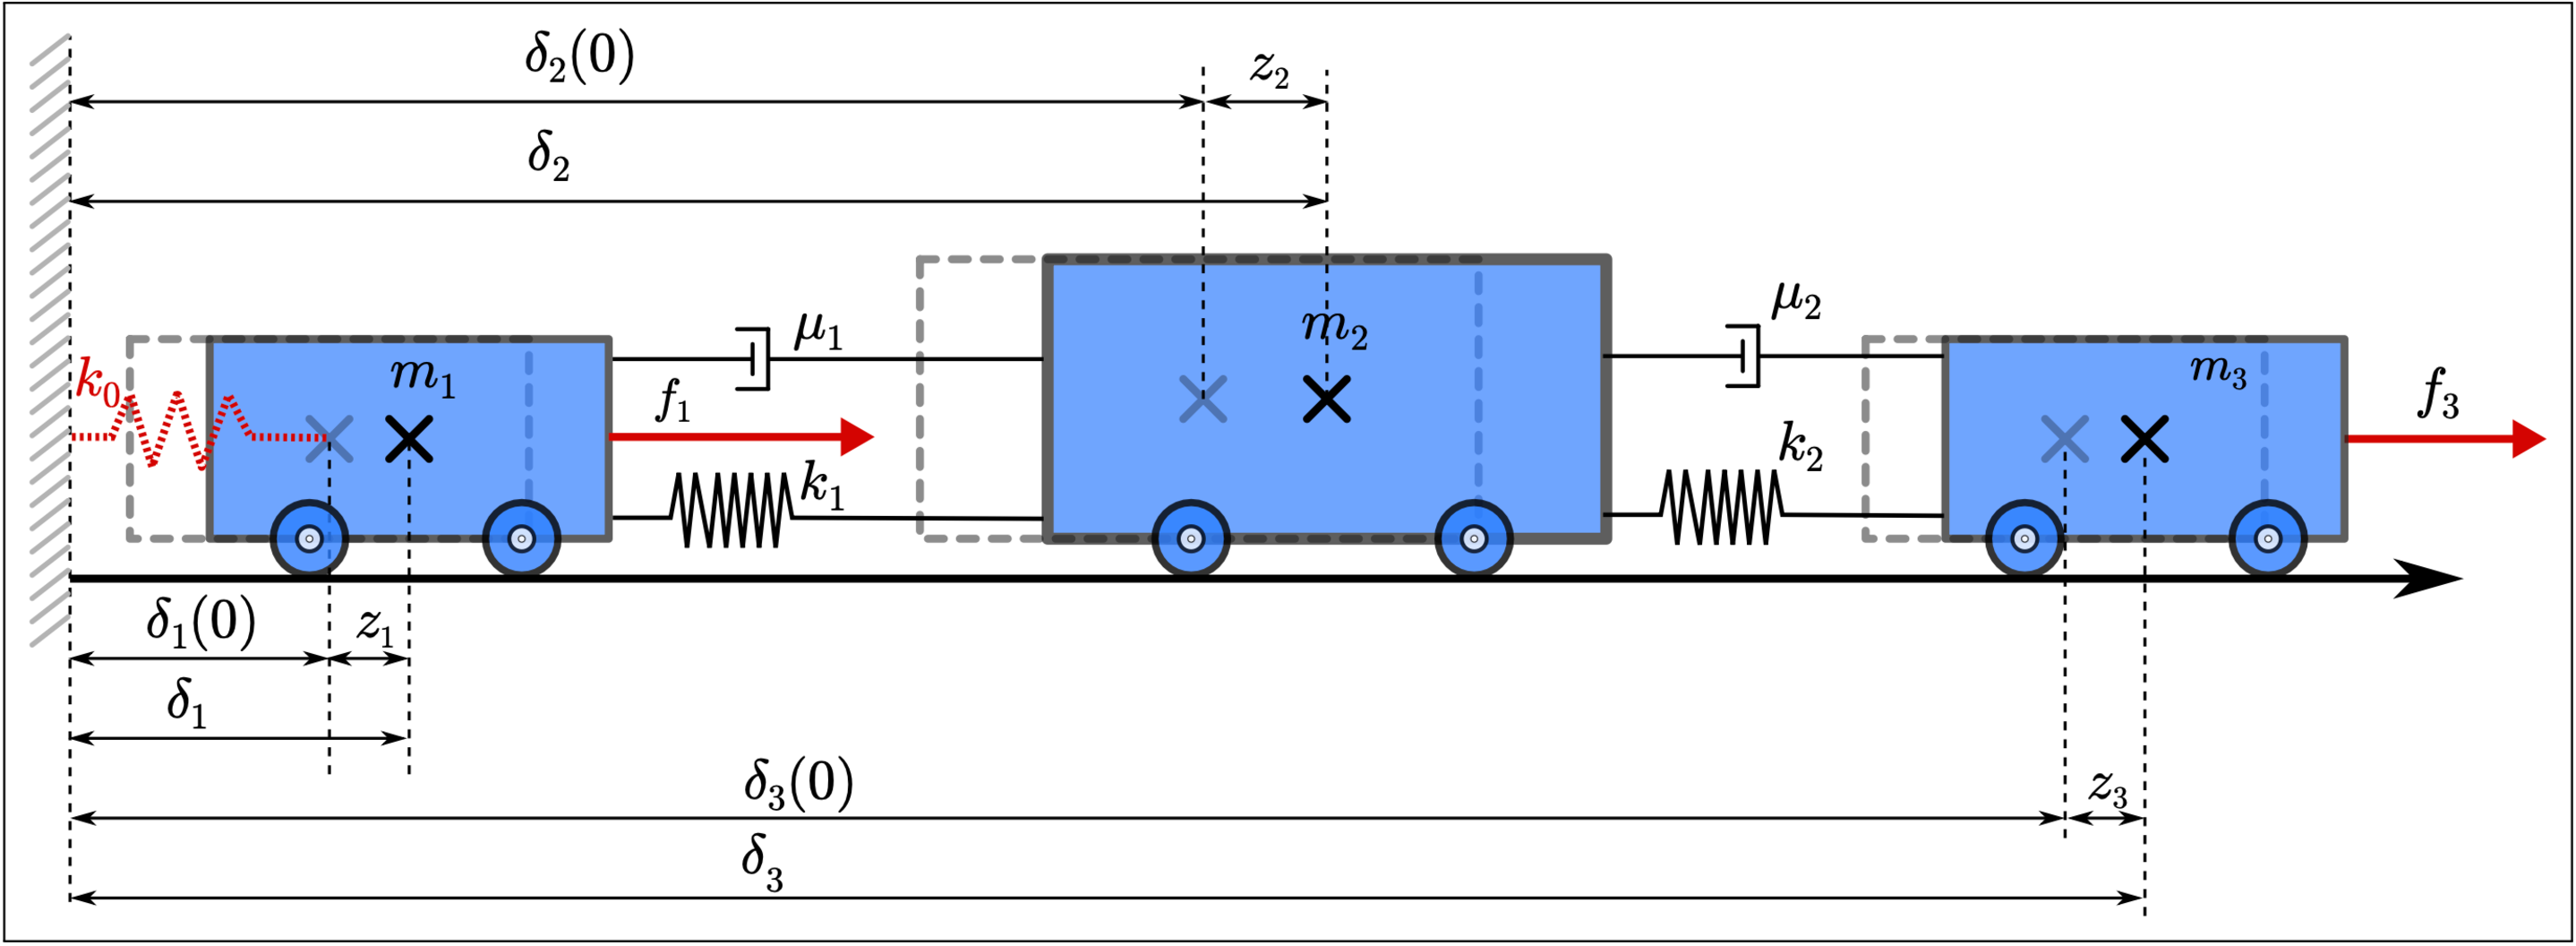
\includegraphics[width=\textwidth]{Figures/3MSD.pdf}
    \caption*{3-MSD System}
\end{figure*}\\
All system's parameters are specified in the Matlab file. 
We firstly study nominal performance (and stability) and then move to robust stability.
\subsection{Nominal Performance Formulation}
We assume we want to control the position of the first and third mass and \textbf{assign them a constant reference} $r = [0.5,1.5]^T$. Notice that this reference is on the relative displacement, which is our measurable output $y = [z_1, z_3]^T$.
\\We also assume the presence of high frequency measurement noise $n$ on all $y_i$ and a constant disturbance $-\Bar{d_1}$ opposing the movement acting on the first mass due to some wheel malfunctioning.
\clearpage
\subsubsection{Augmented Plant}
The augmented plant used can be visualized like this:
\begin{figure}[h!]
    \FigureEight
    \caption{Triple SMD Augmented Plant}
    \label{fig:fig08}
\end{figure}
\\With $G_d$ being a \textbf{selection matrix} (disturbance only acts on first mass), $w_S(s),\ w_U(s)$ being performance weights for the sensitivity and control sensitivity respectively, and finally $D_n$ a scaling matrix needed just for synthesis. 
\\Notice that in the actual simulation scheme, only the selection matrix $G_d$ is kept, while for the controller synthesis with $hinfsyn(\dots)$, all weights must be used.
\subsubsection{Controller Synthesis}
We used two controllers to solve the nominal performance Problem: one designed on the Augmented Plant with $hinfsyn(\dots)$ and the second designed with $mixsyn(\dots)$ on the nominal plant $G(s)$.
\\
A comparison in terms of tracking and control effort can be seen in Fig.~\ref{fig:fig09}. We can observe similar tracking performances but significantly different control efforts. The controller designed on the augmented plant seems to have lower bandwidth since it exhibits a much lower peak and is much less sensitive to measurement noise. In the graph relative to the other controller, on the other hand, we can clearly see the "sawtooth" shape in the control effort, meaning our controller is very responsive but doesn't reject the measurement noise.
\\For these reasons, \textbf{the controller designed on the augmented plant is more performant} and will be used for studying robust stability.
\clearpage
\begin{figure}[h!]{}
    \begin{subfigure}[t]{0.45\textwidth}
    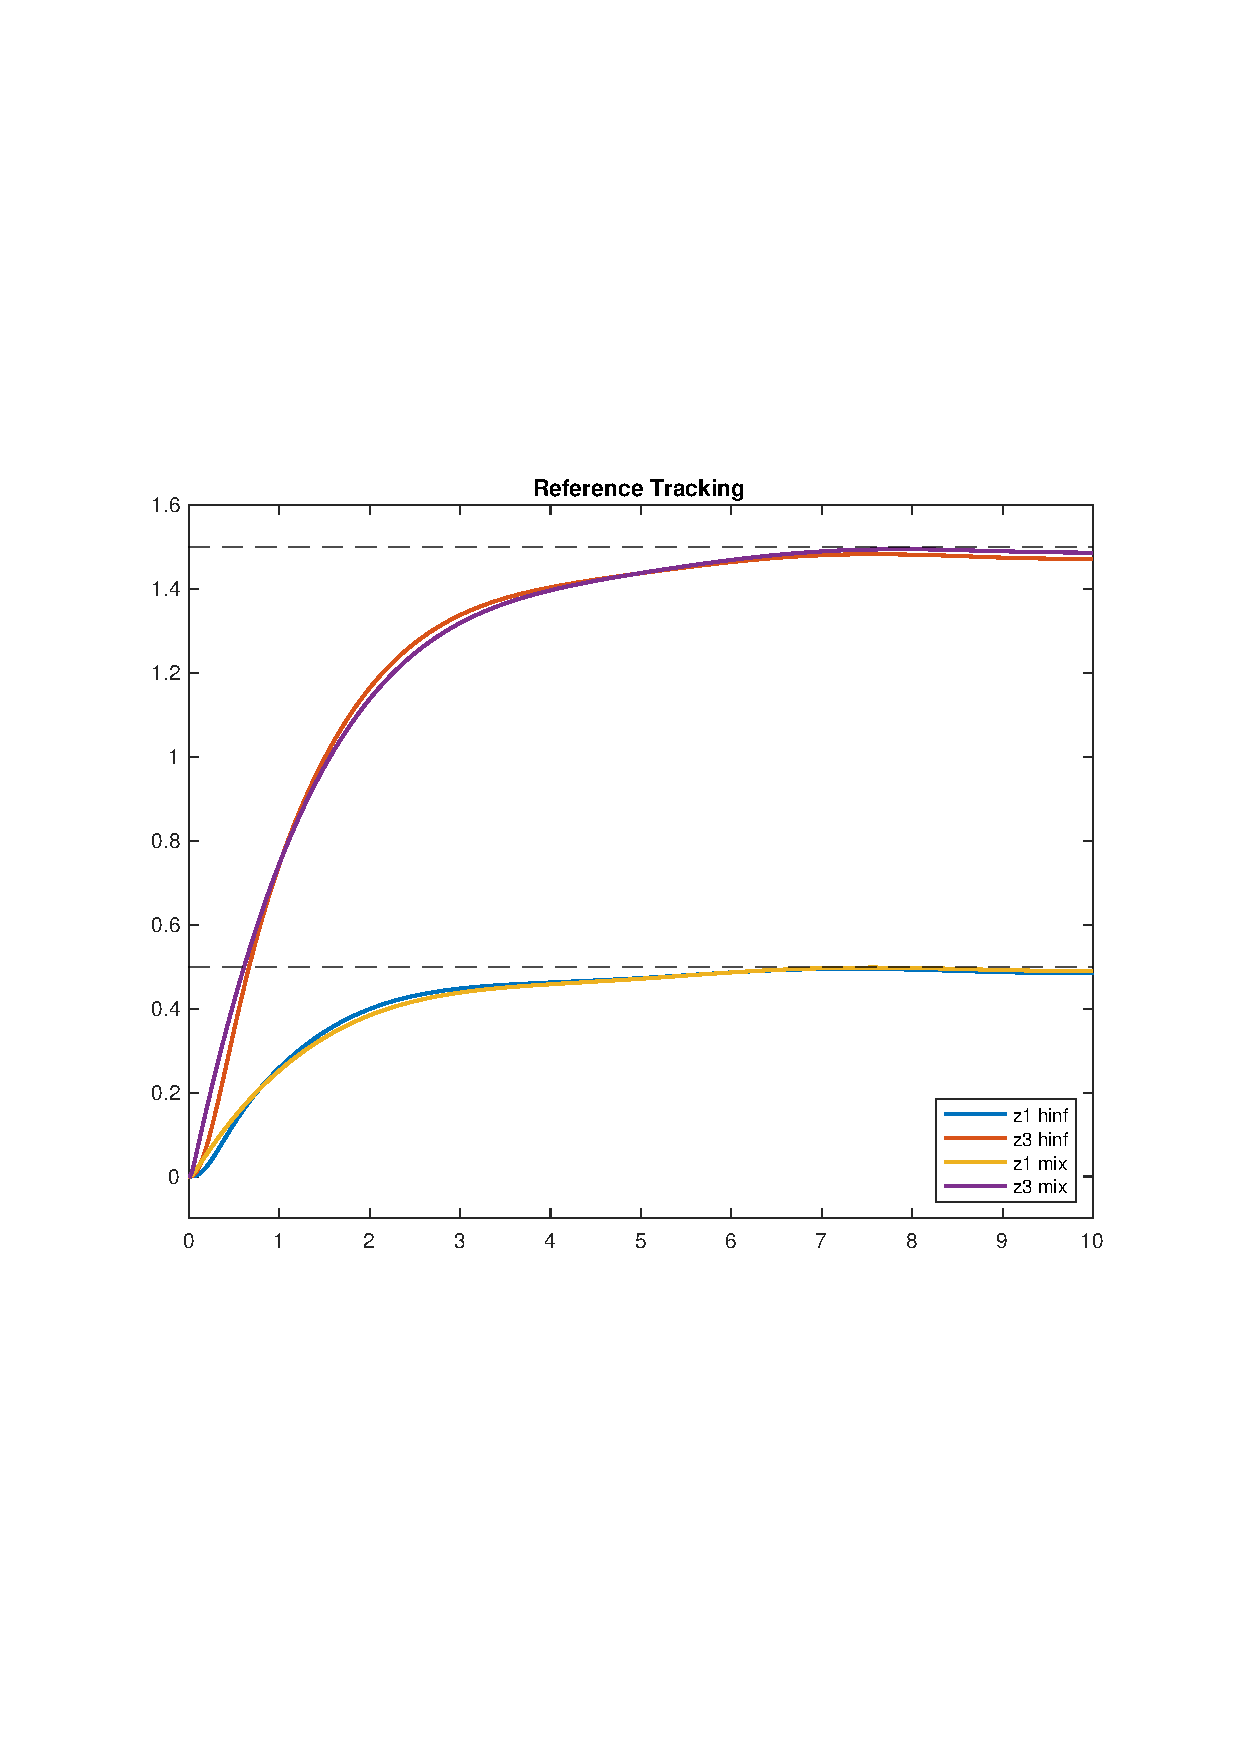
\includegraphics[width=\textwidth]{Figures/fig09a.pdf}
           \subcaption{Reference Tracking Comparison}
           \label{fig:fig09a}
    \end{subfigure}
    \begin{subfigure}[t]{0.45\textwidth}
    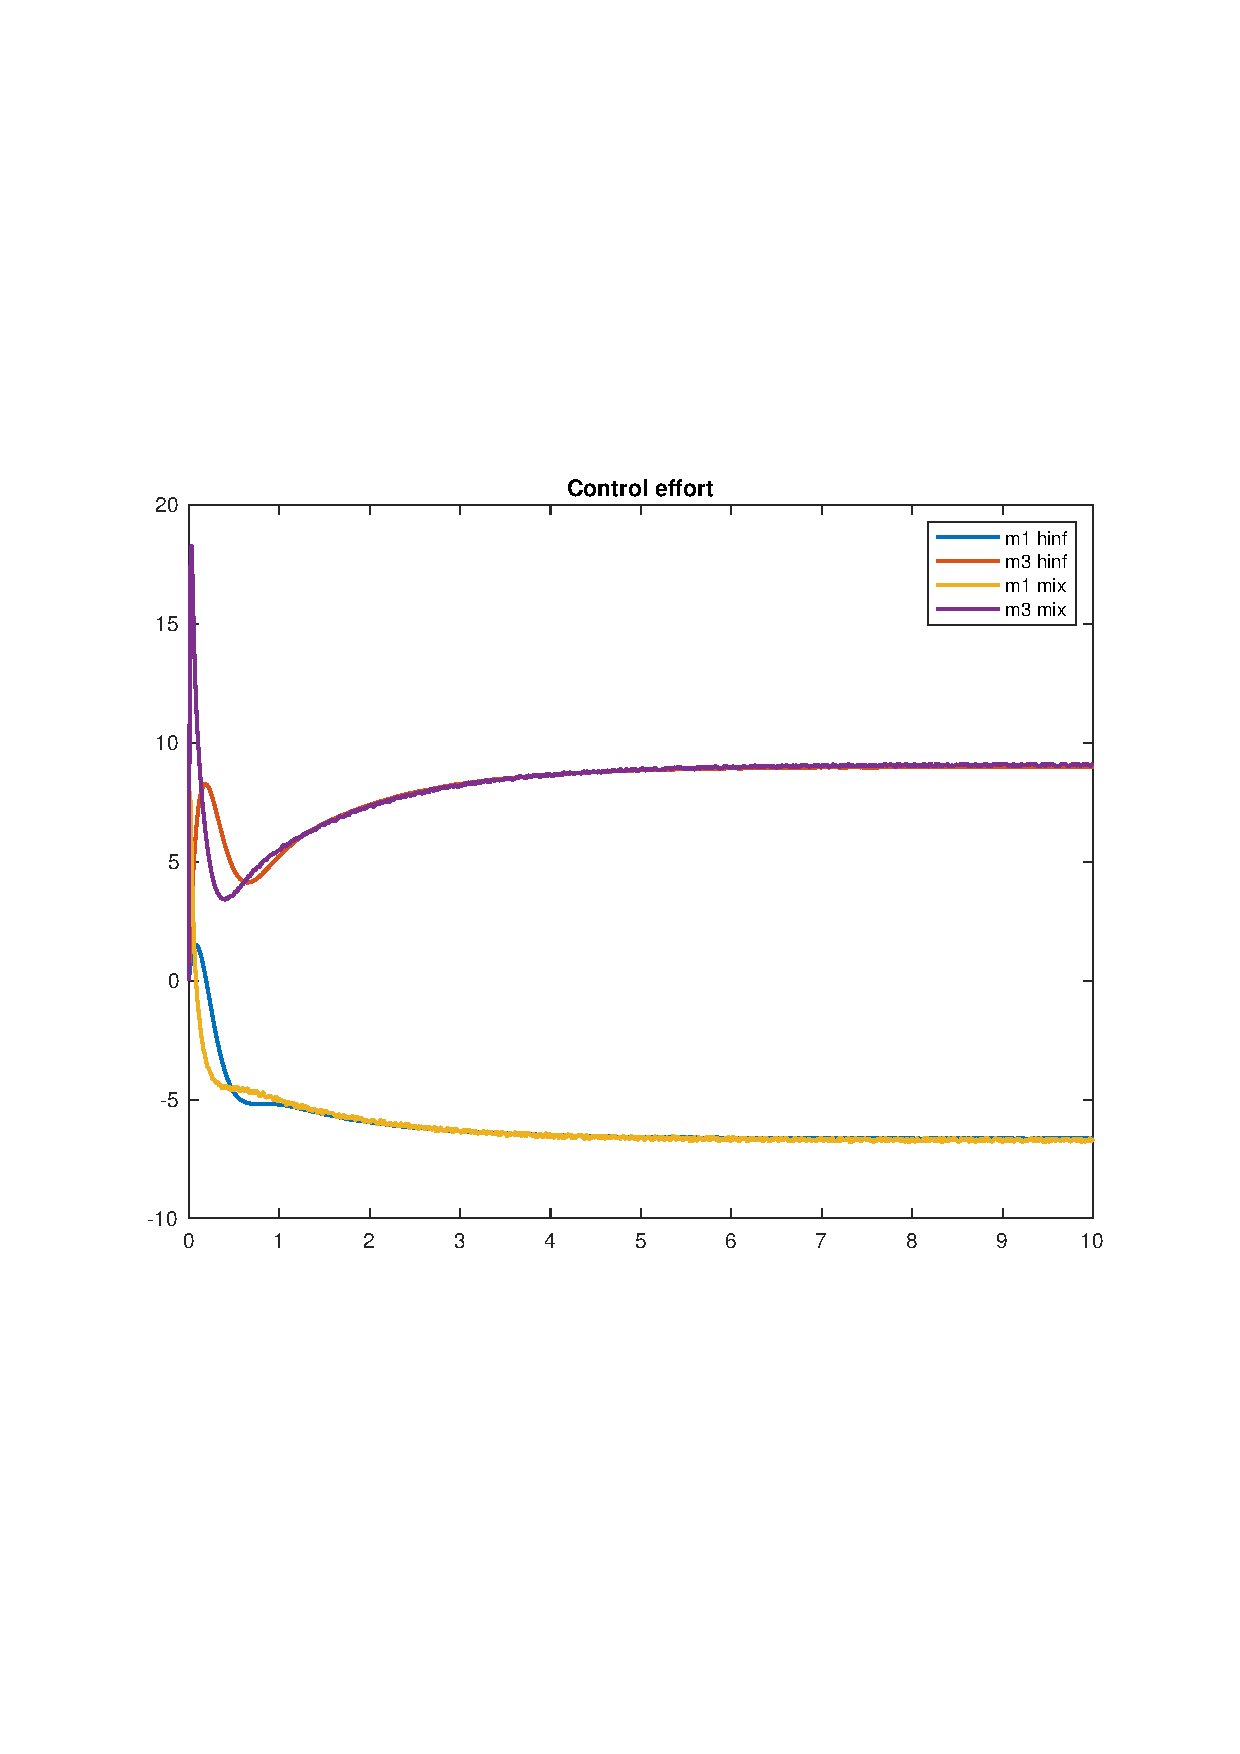
\includegraphics[width=\textwidth]{Figures/fig09b.pdf}
           \subcaption{Control Effort Comparison}
           \label{fig:fig09b}
    \end{subfigure}
    \caption{Controller designed on the augmented Plant vs Regular Plant}
    \label{fig:fig09}
   \end{figure}
\subsection{Robust Stability: Analysis}
Let's now try to add some uncertainty and study robust stability of the $hinfsyn(\dots)$ controller found, using different formulations.
\subsubsection{Uncertainty Definition}
We're going to add a 10\% parametric uncertainty on the three masses $m_1,m_2,m_3$. Therefore the "actual" uncertainty matrix will be structured, real valued and diagonal, but we'll start using the more conservative full complex representation.
\subsubsection{Full Complex Additive Representation}
We consider the uncertainty formulation $G(s) = G_n(s) + \Delta_A(s) w_A(s)$ with $w_A(s)$ the proper weight found with the command $ucover(...)$.\\ \\
Not too surprisingly, the additive formulation is too conservative and the controller is not robustly stabilizing the Plant. In fact, not only the robstab command gives bounds smaller than one, but also the necessary and sufficient condition for robust stability fails: $\|w_a(s) S_o(s)\|_\infty >> 1$

\subsubsection{Full Complex Input Multiplicative Representation}
The Input Multiplicative formulation $G(s) = G_n(s)(I + \Delta_I(s) w_I(s))$, which is still a full complex representation and therefore still very conservative, gives opposite results. N\&S condition holds $\|T_i(s)w_I(s) \|_\infty \approx 0.4 < 1$ and robstab gives bounds greater than one.
\subsubsection{Full Complex Output Multiplicative Representation}
Very similar results hold using the output multiplicative formulation \\ $G(s) = (I + \Delta_O(s) w_O(s))G_n(s)$. We still satisfy the N\&S condition \\$\|T_o(s)w_O(s) \|_\infty \approx 0.35 < 1$ and the robstab conditions.
\subsection*{Remark: MIMO Nyquist Criterion}
A further investigation on robust stability can be performed using the MIMO Nyquist criterion. We consider the function $D(s) = det|I_{2x2} + L_{nom}(s)|$ and verify that there are no encirclements of the origin. 
\\However, $D(s)$ represents the "nominal behavior" and therefore, we need to take into account the "uncertainty discs" at each frequency. The radius of those discs is directly proportional to each weight $w_O=(s), w_I(s), w_A(s)$ and none of the discs should encircle the critical point (0,0).
\\\\In Fig.~\ref{fig:fig10} we can visualize Nyquist plots for the three cases. We see that the blue-dotted discs encircle the origin only in the additive case. Moreover, the disc in green represent the uncertainty at the critical frequency and is the only one which is scaled by the quantity $UpperBound$. 
\\In all cases, such green disc passes through the origin, proving that all plots are consistent.
\begin{figure}[h!]{}
    \begin{subfigure}[t]{0.32\textwidth}
           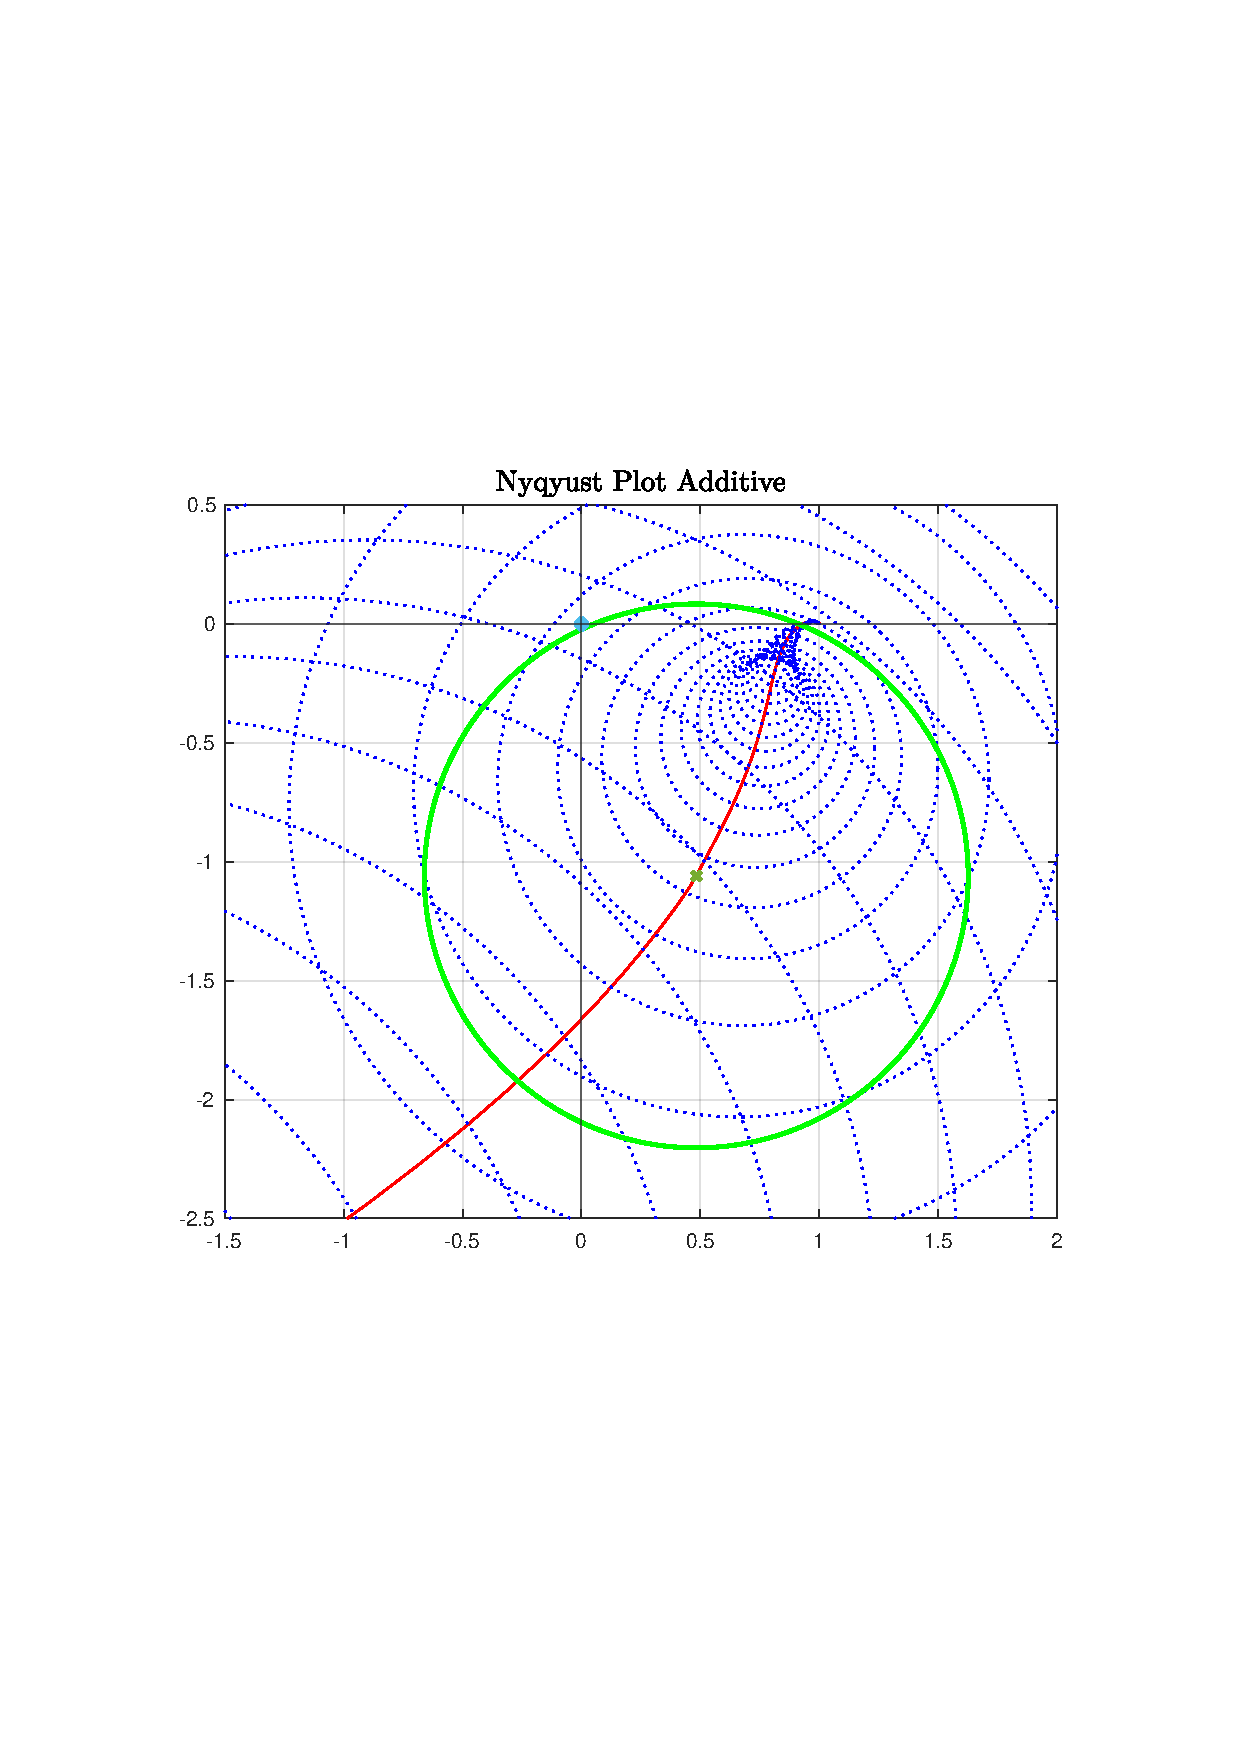
\includegraphics[width=\textwidth]{Figures/fig10a.pdf}
           \subcaption{Additive}
           \label{fig:fig10a}
    \end{subfigure}
    \begin{subfigure}[t]{0.32\textwidth}
           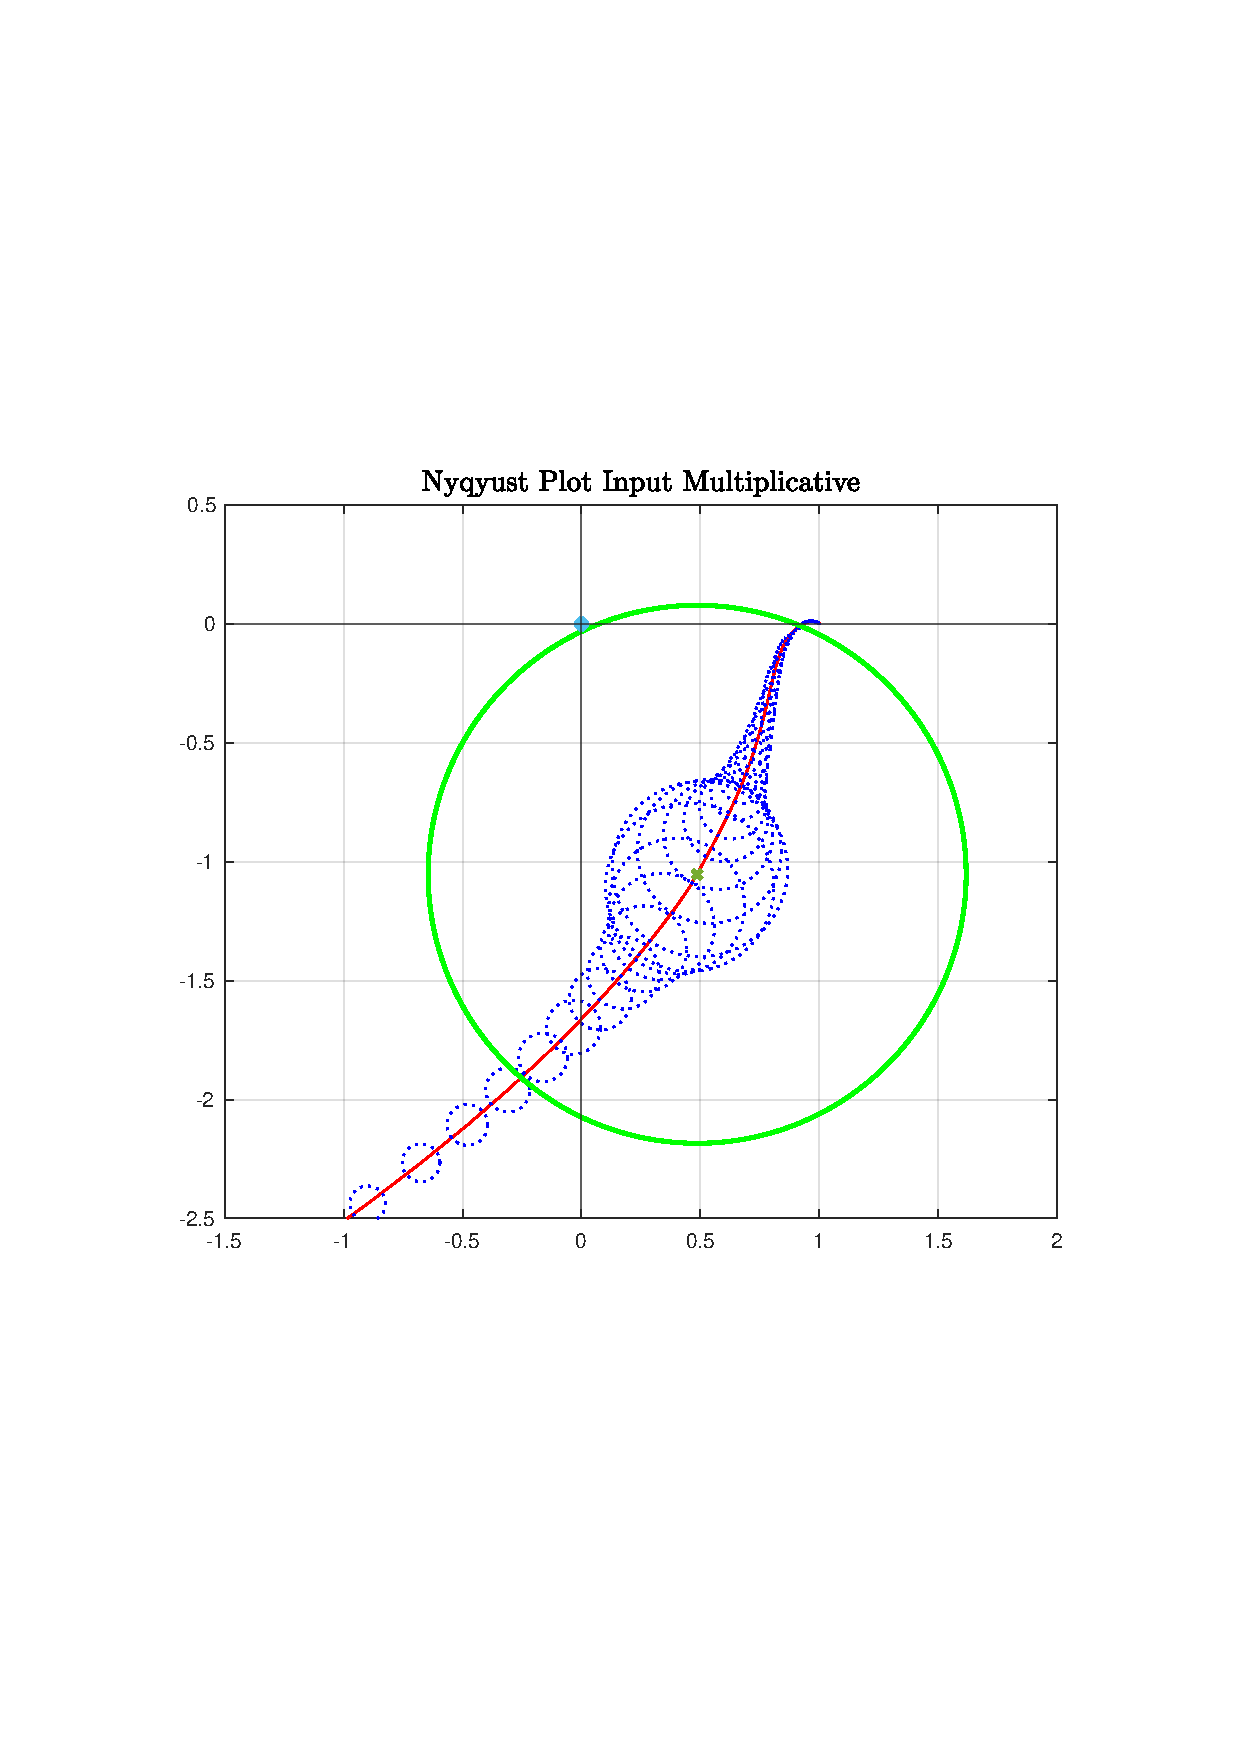
\includegraphics[width=\textwidth]{Figures/fig10b.pdf}
           \subcaption{Input Multiplicative}
           \label{fig:fig10b}
    \end{subfigure}
    \begin{subfigure}[t]{0.32\textwidth}
    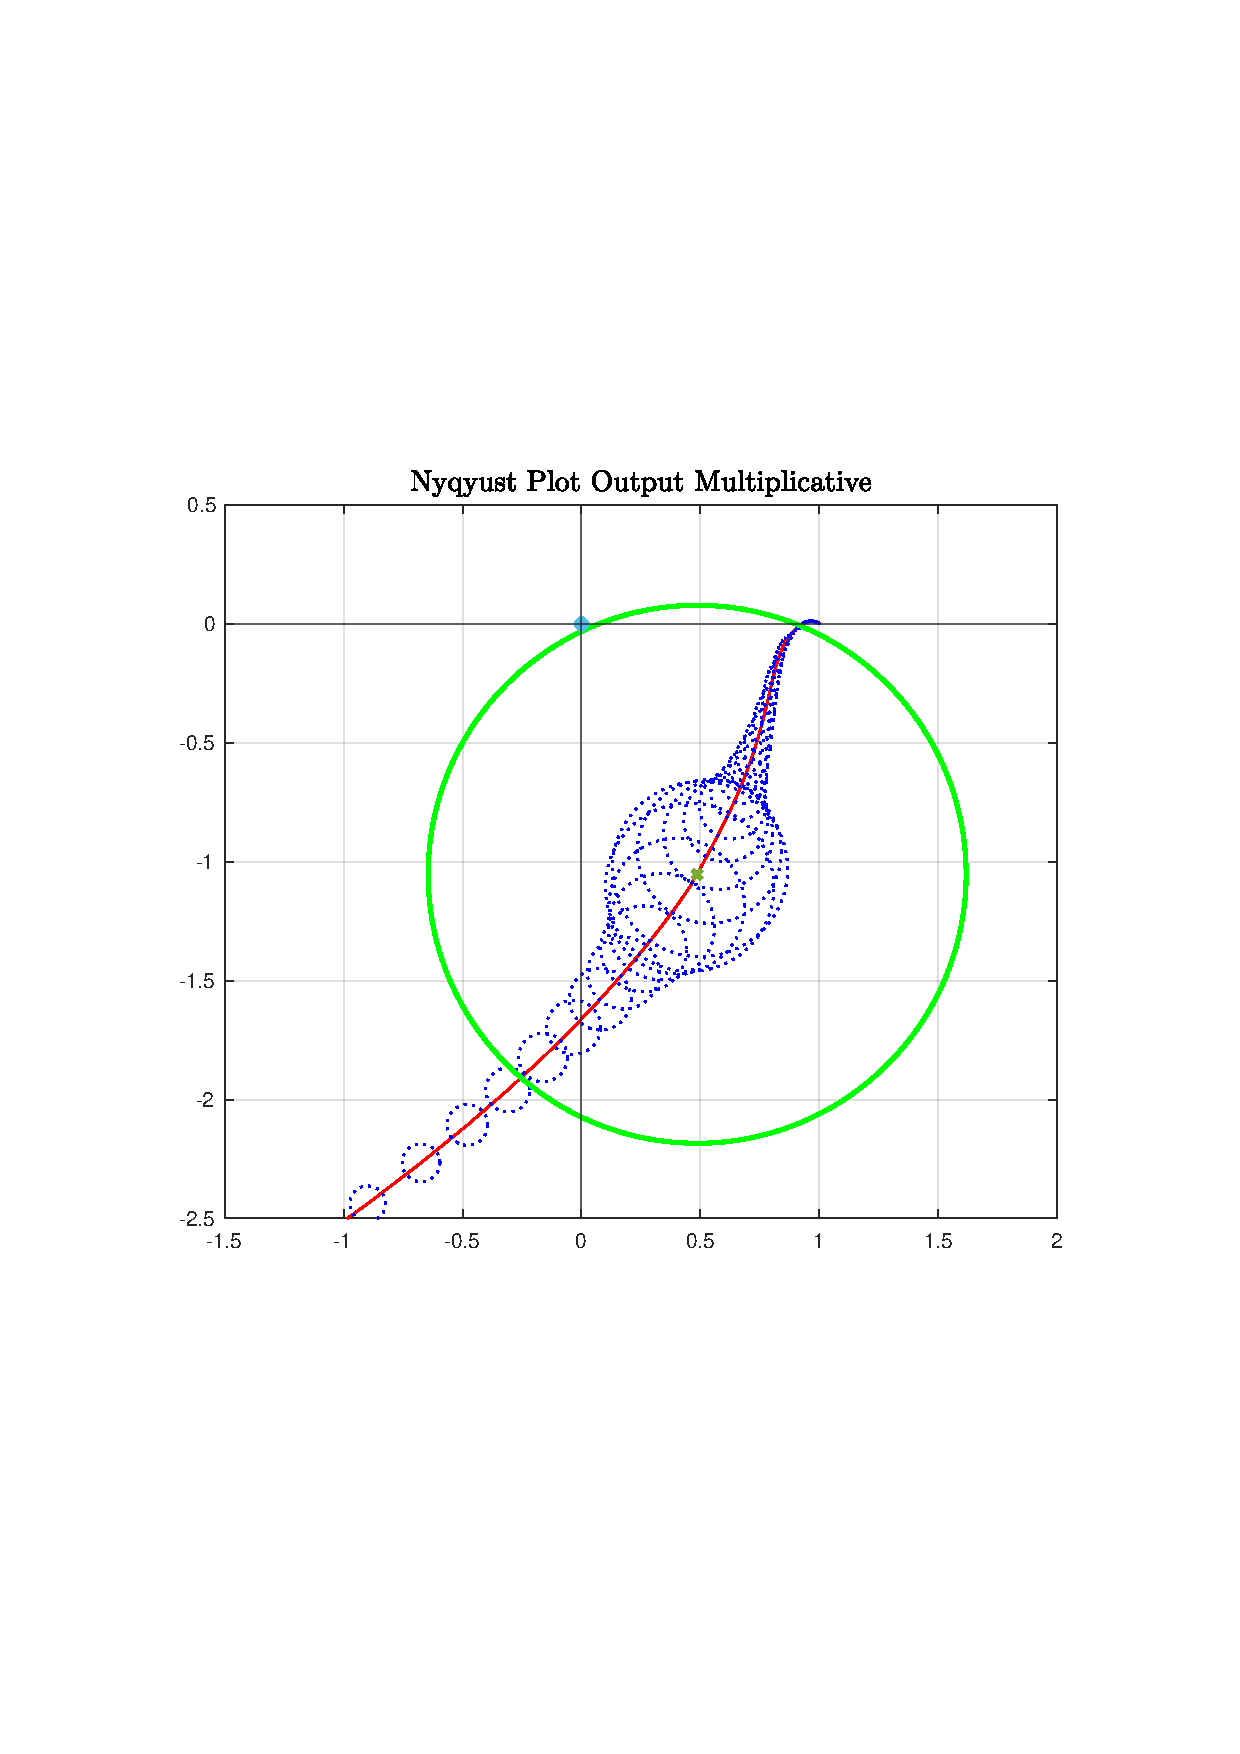
\includegraphics[width=\textwidth]{Figures/fig10c.pdf}
           \subcaption{Output Muliplicative}
           \label{fig:fig10c}
    \end{subfigure}
    \caption{MIMO Nyquist criterion with uncertainty}
    \label{fig:fig10}
   \end{figure}
\clearpage
\subsubsection{Structured Real Uncertainty}
It's no surprise that the least conservative representation leads to robust stability as well. The robstab bounds are the highest of the bunch, meaning the system can "take the most uncertainty" using this real structured representation.
\\\\
However, a more articulated study of robust stability with structured uncertainty will be performed in the next section, using Structured Singular Values.
\subsection{Robust Stability: SSV analysis}
In this section we'll study the SSV of the uncertain plant. However, we'll also use $\mu$-synthesized controller as a reference to confront it with the $hinfsyn()$ controller.
\subsubsection{SSV for the Augmented Plant (structured uncertainty)}
For starters, we consider the full augmented plant as in Fig.~\ref{fig:fig08}, but instead of the nominal plant $G(s)$ we consider the uncertain one $G_{unc}(s)$. 
We therefore consider in the scheme all the performance weights and the nominal controller.
\\\\ As a \textbf{first step we now need to "pull out" the uncertainty}. This is done on the Matlab file using the command $lftdata(...)$ on the uncertain plant. For our system, the uncertainty will be a real diagonal matrix 
$\Delta = \begin{bmatrix}
\delta_1 & 0 & 0\\
0 & \delta_2 & 0\\
0 & 0 & \delta_3
\end{bmatrix}$ in which each $\delta_i$ term represents the uncertainty of the $m_i$ mass and is such that $\|\delta_i(j\omega)\|_\infty < 1$. 
\\\\
The obtained control scheme can be visualized as the following:
\begin{figure*}[h!]
\centering
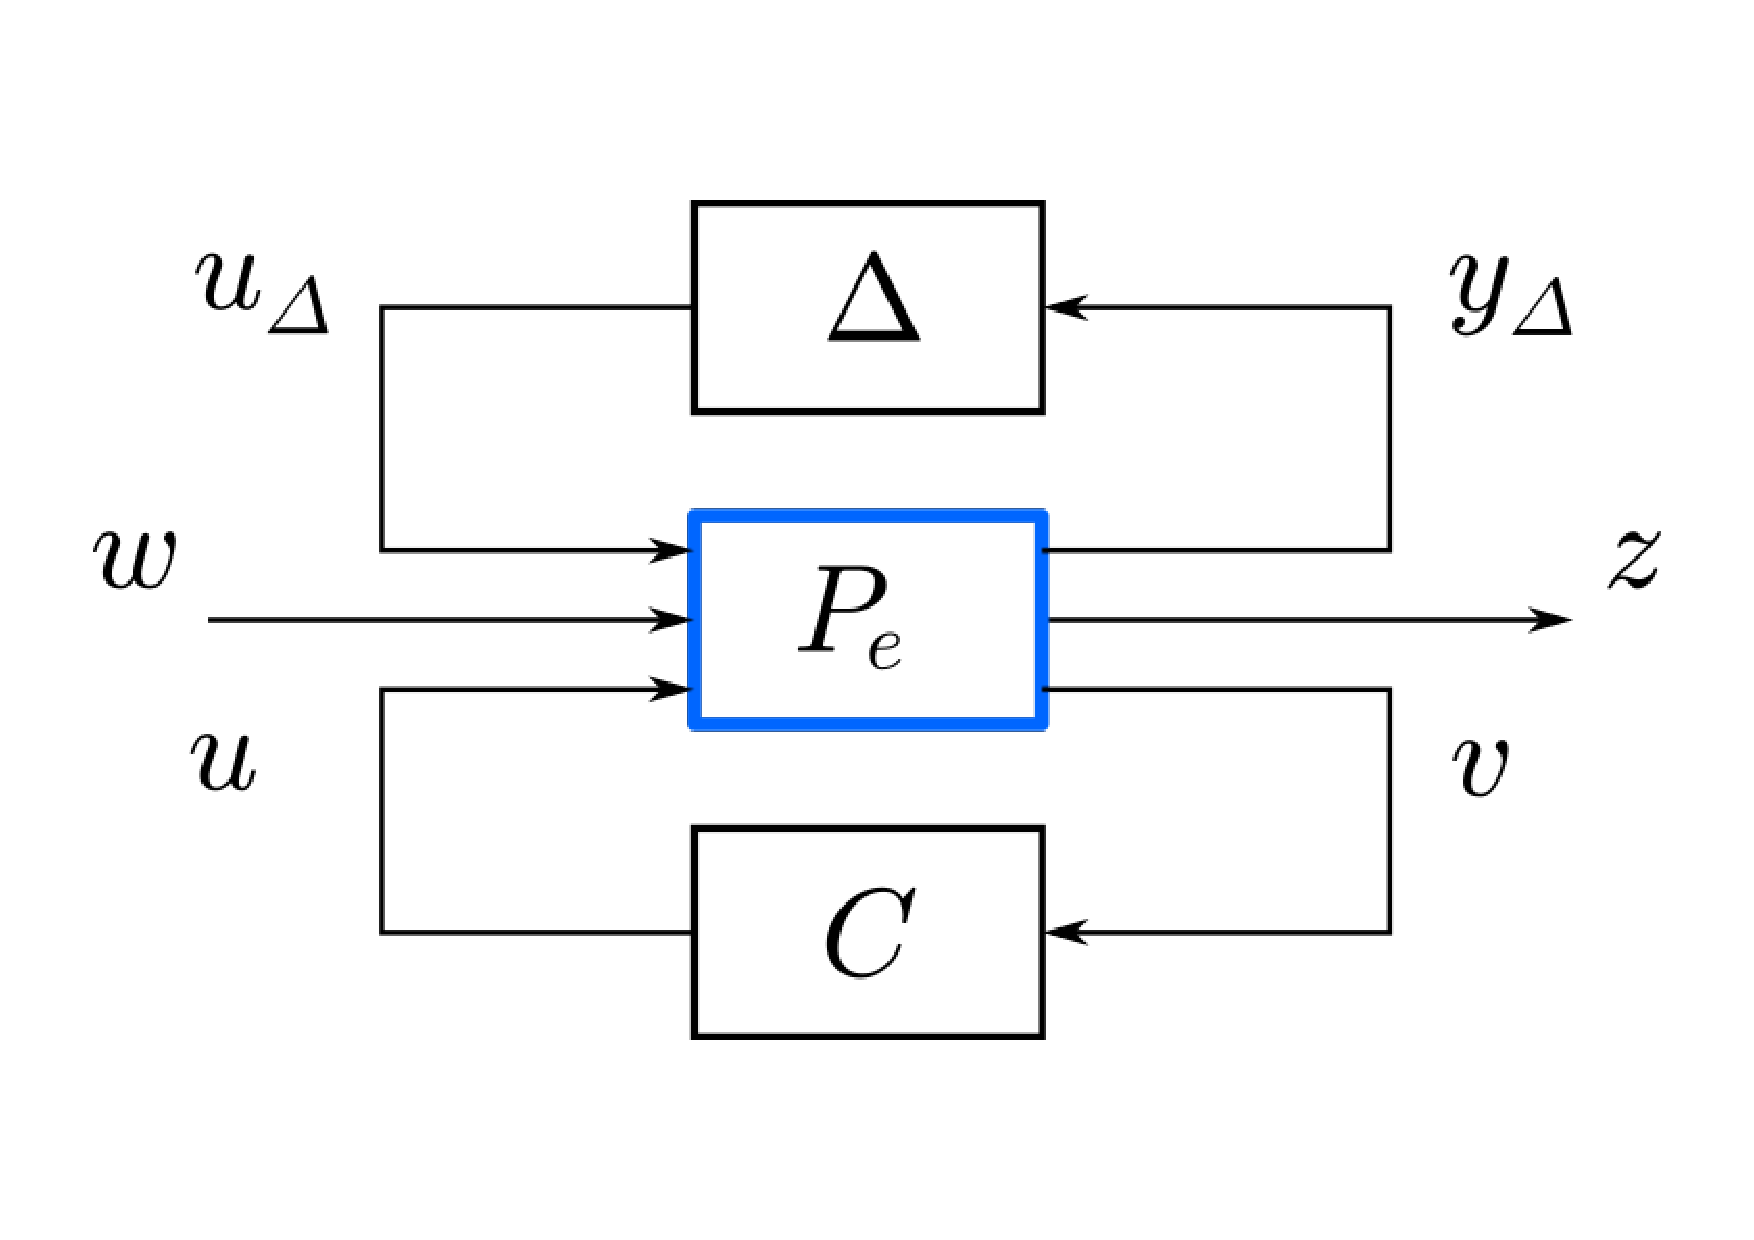
\includegraphics[width=0.5\textwidth]{Figures/extra01.pdf}
\end{figure*}\\
We can now proceed with closing the controller loop with the lower lft and consider the resulting $N = F_\ell (P_e,C)$. \\
We know that the only part of the lft that may lead to instability is the term $\Psi = (I-N_{11}\Delta)^{-1}$, since every other term can be seen as a series-like interconnection of asymptotically stable "terms".
\\\\
Such term itself can be seen as a positive feedback interconnection between the $N_{11}$ (usually called $M$) term and the uncertainty $\Delta$, in what is typically called the $M-\Delta$ scheme.\\
\\We can therefore consider the MIMO Nyquist Criterion for $\Psi$ and look for the smallest destabilizing $\delta_{min}\ s.t.\ det|\Psi| = 0$. If such  $\delta_{min} > 1,\ \forall \omega$ then we can conclude on Robust Asymptotic Stability.
\\ Taking the reciprocal of the same relation, we get the $\mu$ notation with the Structured Singular Values, and we get the equivalent formulation:
\begin{equation*}
\sup_{\forall \omega} \left| \mu_{\Delta} (M) \right| < 1
\end{equation*}
\\
Notice that when considering an unstructured, full complex uncertainty we have that $\Bar{\sigma}(M) \equiv \mu_{\Delta} (M)$.
\\
It the plot below we see the structured singular values of our $M(s)$-$\Delta$ scheme.
\begin{figure}[h!]
    \FigureEleven
    \caption{SSV with 10\% and 40\% uncertainty on masses}
    \label{fig:fig11}
\end{figure}
\\We notice that our system can "still take" much uncertainty: even quadrupling all uncertainty (up to 40\%) we still obtain robust stability
\clearpage
\subsubsection{Controller $\mu$-synthesis}
Just for reference, we can use the usual augmented Plant in Fig.~\ref{fig:fig08} to perform $\mu$-synthesis control and analyze nominal performance and robust stability. We notice the presence of oscillatory transient behavior, which is however justified by the nature of the physical system. Moreover, this controller requires much less control effort than the one designed with $mixsyn()$ (designed only on the plant, not the augmented plant). It is also less sensitive to noise than the other two, due to lower bandwidth.
More importantly for our analysis, stability margins are further improved, as testified by both the $robstab(\dots)$ bounds and the SSV plot.
\begin{figure}[h!]{}
    \centering
    \begin{subfigure}[t]{0.45\textwidth}
    \FigureTwelveA
    \subcaption{Nominal Performance:
    \\ Tracking}
    \label{fig:fig12a}
    \end{subfigure}
    \begin{subfigure}[t]{0.45\textwidth}
    \FigureTwelveB
       \subcaption{Nominal Performance:
    \\ Contrl Effort}
       \label{fig:fig12b}
    \end{subfigure}
    \begin{subfigure}[t]
    {0.7\textwidth}
    \FigureTwelveC
           \subcaption{Robust Stability:
    \\ SSV plot}
    \end{subfigure}
    \caption{$\mu$ controller: Nominal Performance and Robust Stability comparison}
    \label{fig:fig12}
   \end{figure}
\end{document}